\chapter{HASIL DAN PEMBAHASAN}
Pada bab ini akan dibahas hasil evaluasi terhadap model dan pengujian sistem. Evaluasi terkait model diantaranya evaluasi deteksi tangan, evaluasi pengenalan gestur tangan dan pengujian SNR. Pengujian terhadap subjek diantaranya pengujian deteksi tangan menggunakan retinex, pengujian pengenalan destur tangan menggunakan Retinex serta pengujinan sistem secara keseluruhan.

Evaluasi terkait model digunakan untuk menilai suatu model yang akan digunakan dalam pengujian terhadap subjek. Model deteksi tangan akan dievaluasi menggunakan mAP, sedangkan model pengenalan gestur akan dievaluasi dengan \textit{k-fold cross-validation}, kemudian untuk mengevaluasi Retinex menggunakan perbandingan SNR.

Pengujian sistem dibagi menjadi 3 yaitu pengujian deteksi tangan, pengujian pengenalan gestur tangan dan pengujian sistem keseluruhan. Setiap pengujian tersebut akan dibandingkan ketika menggunakan retinex dan tanpa menggunakan Retinex. Pengujian dilakukan oleh 3 subjek yang berbeda di luar dari dataset.
\section{Evaluasi Deteksi Tangan}
Pengujian mAP dari dilakukan dengan skema pada gambar 6.1. Hasil anotasi setiap citra dataset maupun citra prediksi akan diekstrak menjadi format file txt dimana berisi nilai koordinat dari citra. Citra yang akan dilakukan prediksi adalah citra dataset testing yang berjumlah 200 citra. Nilai mAP merupakan hasil rata rata dari setiap \textit{Average Precicion}, dimana variasi IOU 0,5 hingga 0,95 dengan 0,05 setiap stepnya. Hasil pengujian mAP ditunjukan pada tabel 6.1 dengan nilai mAP sebesar 50,62. Hasil dari pelatihan deteksi objek ini akan digunakan sebagai model pada sistem.
Penelitian yang dilakukan dengan dataset COCO memperoleh hasil mAP sebesar 22,1. 
\begin{table}[H]
	\caption{Evaluasi mAP Model Object Detection}
	\vspace{0cm}
	\centering
	\begin{tabular}{|c|c|c|c|c|c|c|c|c|c|}
		\hline \multicolumn{10}{|c|}{Mean Average Precicion(mAP) = 50,62} \\ 
		\hline @0,5 &  @0,55 &@0,60 & @0,65 &@0,70&@0,75&@0,80&@0,85&@0,90&@0,95\\
		\hline  76,58& 76,58 &74,72 &73,34 &63,85 & 46,3&29,12 & 19,76&3,64 &0,02 \\ 
		\hline
	\end{tabular}
\end{table}

\section{Evaluasi Pengenalan Gestur Tangan}
\section{Pengujian SNR}
Pengujian SNR dilakukan dengan membandingkan 2 algoritma Retinex dengan citra asli. Citra yang akan digunakan pada pengujian SNR diambil dari 3 kondisi citra yang mewakili intensitas yang digunakan. Nilai parameter Retinex yang akan digunakan merujuk dalam pengujian ini merujuk pada penelitian yang dilakukan oleh (Petro, 2014) dan 2 variasi nilai parameter yang ditentukan oleh peneliti. Nilai yang di gunakan untuk mengisi parameter Retinex ditunjukan pada tabel 6.2.
\begin{table}[H]
	\caption{Parameter Nilai Retinex}
	\vspace{0cm}
	\centering
	\begin{tabular}{|c|c|c|c|c|c|} 
		\hline  Parameter&$\sigma_{1}$ & $\sigma_{2}$ &$\sigma_{3}$ &$\alpha$ &$\beta$\\
		\hline  Petro, 2014&15& 80 &250 & 125& 46\\ 
		\hline  Variasi 1&10 &60&180&100&30\\
		\hline	Variasi 2&30&100&210&140&60\\
		\hline
	\end{tabular}
\end{table}
\noindent Citra yang yang dilakukan operasi Retinex akan di lanjutkan dengan operasi deteksi tangan, kemudian di lakukan perbandingan dengan waktu komputasi, hasil deteksi dan nilai PSNR untuk menentukan Retinex yang akan dipakai.

Hasil perbandingan citra Retinex ditunjukan pada gambar 6.1, 6.2, dan 6.3. Secara visual citra asli setelah dilakukan operasi Retinex terjadi peningkatan terhadap kecerahan, sehingga detail dari citra lebih dapat terlihat daripada citra asli. Citra asli terdapat pada baris pertama, kemudian citra \textit{Multiscale Retinex} pada baris kedua dan citra \textit{Multiscale Retinex Color Restoration} pada baris ketiga. Seluruh citra yang dikenai Retinex telah dilakukan proses deteksi tangan.
% TODO: \usepackage{graphicx} required
\begin{figure}[H]
	\centering
	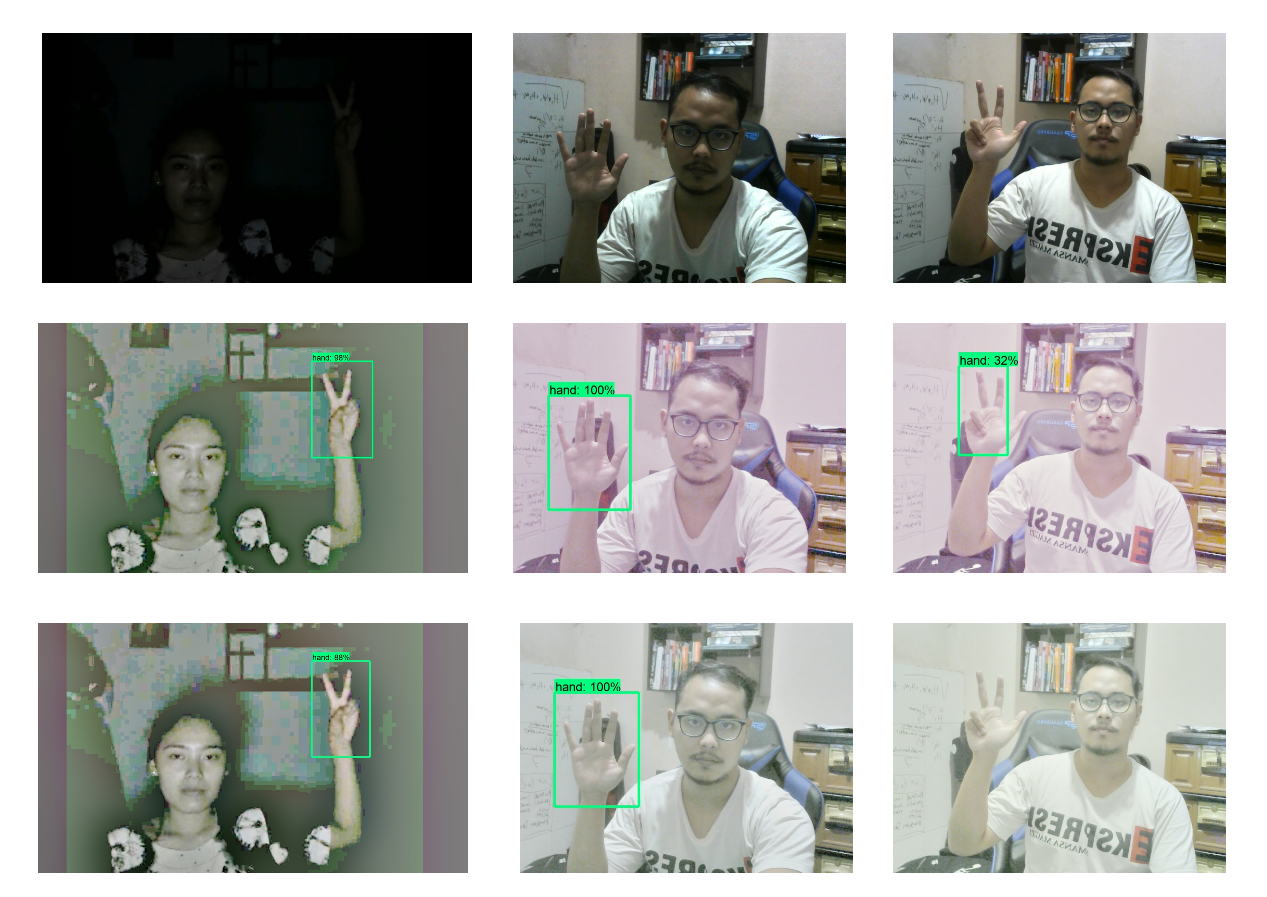
\includegraphics[width=0.9\linewidth]{ps}
	\caption{Perbandingan Hasil Citra Retinex Parameter Petro, 2014.}
	\label{fig:ps}
\end{figure}
\begin{figure}[H]
	\centering
	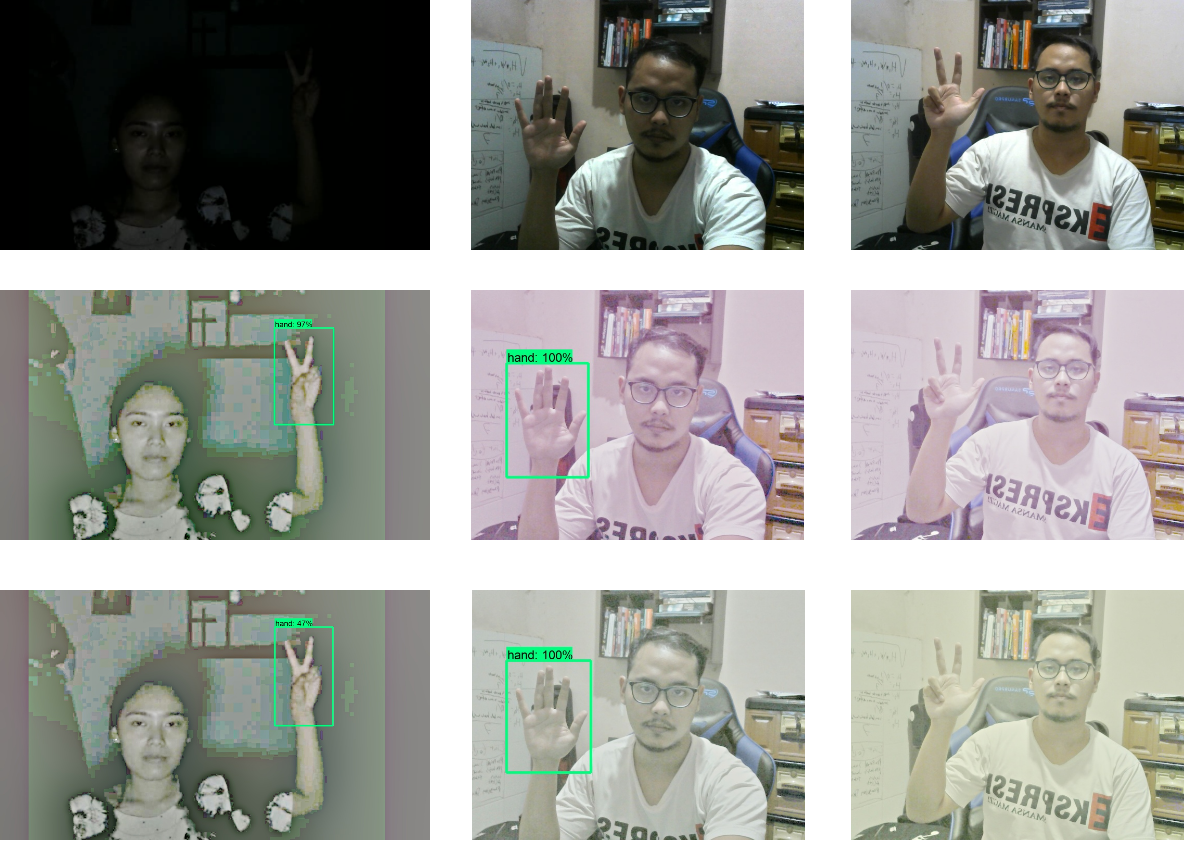
\includegraphics[width=0.85\linewidth]{versi1}
	\caption{Perbandingan Hasil Citra Retinex Parameter Variasi 1.}
	\label{fig:ps}
\end{figure}
\begin{figure}[H]
	\centering
	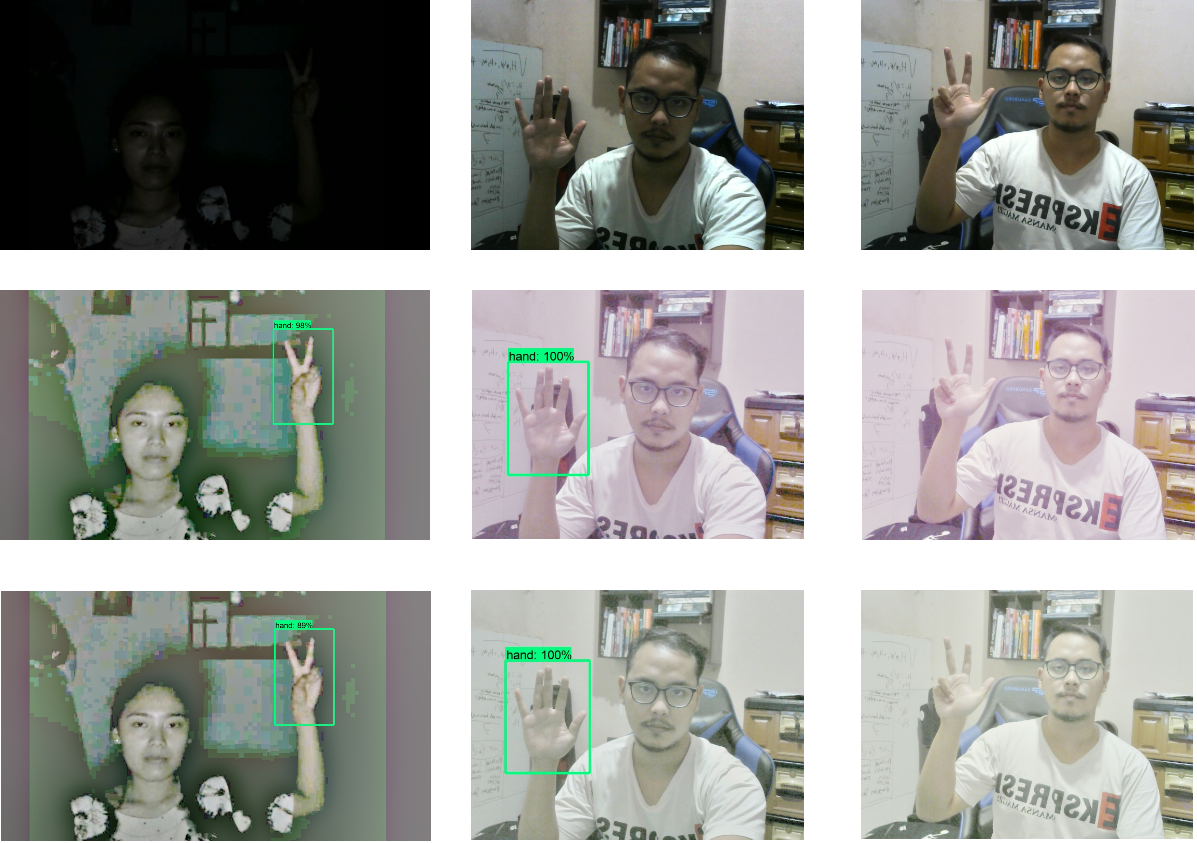
\includegraphics[width=0.85\linewidth]{versi2}
	\caption{Perbandingan Hasil Citra Retinex Parameter Variasi 2.}
	\label{fig:ps}
\end{figure}
Peneliti meninjau kedua algoritma Retinex terkait dengan waktu komputasi dan akurasi dalam melakukan deteksi tangan dan nilai PSNR. Tujuan dari peninjauan ini dilakukan untuk memilih algoritma Retinex yang efektif. Hasil Tabel 6.3 merupakan pengujian PSNR, dari data tersebut untuk citra1 dimana kondisi citra sangat gelap MSR lebih unggul akan tetapi nilai yang yang dihasilkan tidak terlalu signifikan antara kedua metode. Citra2 dan citra 3 memiliki selisih 0.94 dan 0.575, dimana MSRCR lebih unggul pada kondisi tersebut untuk parameter Petro. Kondisi cahaya yang semakin terang meningkatkan nilai PSNR pada MSRCR untuk ketiga variasi parameter.
\begin{table}[H]
	\caption{Hasil Pengujian PSNR}
	\vspace{0cm}
	\centering
	\begin{tabular}{|c|c|c|c|c|c|c|c|c|c|c|c|c|}
		\hline
		\multicolumn{3}{|c|}{Petro, 2014} &\multicolumn{2}{|c|}{Variasi 1}&\multicolumn{2}{|c|}{Variasi 2} \\
		\hline   &MSR &MSRCR &MSR&MSRCR&MSR&MSRCR\\
		\hline  Citra1 & 6,692&6,688 &6,163 &6,11 &6,657 &6,19 \\
		\hline   Citra2 & 8,23&8,805 &8,497 &9,367 &8,75 &9,41\\
		\hline Citra3 & 9,472& 10,412&9,7 &10,79 & 9,69&10,462\\
		\hline
	\end{tabular}
\end{table}
\begin{table}[H]
	\caption{Perbandingan Nilai Deteksi}
	\vspace{0cm}
	\centering
	\begin{tabular}{|c|c|c|c|c|c|c|c|c|c|c|c|c|}
	\hline
	\multicolumn{3}{|c|}{Petro, 2014} &\multicolumn{2}{|c|}{Variasi 1}&\multicolumn{2}{|c|}{Variasi 2} \\
	\hline   &MSR &MSRCR &MSR&MSRCR&MSR&MSRCR\\
	\hline  Citra1 & 98\%&88\%&97\% &47\% &98\% &89\% \\
	\hline   Citra2 & 100\%&100\% &100\% &100\% &100\% &100\%\\
	\hline Citra3 & 32\%& 0\% & 0\%&0\% &0\% &0\%\\
	\hline
	\end{tabular}
\end{table}
Tabel 6.4 merupakan nilai \textit{confidence} atau nilai deteksi dari hasil deteksi ketiga citra. Hasil tersebut menunjukan bahwa citra yang dikenai MSR memiliki nilai yang lebih tinggi untuk ketiga parameter. Kondisi citra pertama dan kedua dapat dikenali dengan baik oleh semua parameter, namun MSR memiliki nilai yang lebih besar. Kondisi citra ketiga tidak dapat di deteksi oleh MSRCR pada semua variasi parameter, namun MSR dapat mendeteksi dengan nilai 32\% pada parameter Petro. Tabel 6.5 menunjukan waktu komputasi dari suatu Retinex dalam memproses satu citra. Waktu komputasi MSR lebih cepat dibandingkan dengan MSRCR pada citra kondisi gelap, namun semakin terang intensitas citra nilai MSRCR semakin lebih cepat dibandingkan MSR. Selisih waktu komputasi citra tidak terlalu jauh pada setiap variasi parameter yang diujikan. Selisih tertinggi pada parameter variasi 1 citra gelap yang memiliki selisih 1,28 detik. 
\begin{table}[H]
	\caption{Waktu Komputasi Retinex}
	\vspace{0cm}
	\centering
	\begin{tabular}{|c|c|c|c|c|c|c|c|c|c|c|c|c|}
		\hline
		\multicolumn{3}{|c|}{Petro, 2014} &\multicolumn{2}{|c|}{Variasi 1}&\multicolumn{2}{|c|}{Variasi 2} \\
		\hline   &MSR &MSRCR &MSR&MSRCR&MSR&MSRCR\\
		\hline   Citra1 & 10,257s&11,121s&13,2s &14,48s &17s &17,05s \\
		\hline   Citra2 & 7,172s&7,234s &6,41s &6,14s &7,75s &7,357s\\
		\hline Citra3 & 6,795s& 7,367s &6,2s &6,46s &7,366 &7,37s\\
		\hline
	\end{tabular}
\end{table}
Berdasarkan hasil ketiga tabel perbandingan tersebut dengan mempertimbangkan antara PSNR, waktu komputasi dan nilai deteksi pada setiap variasi parameter, maka penelitian ini menggunakan MSR sebagai Retinex yang dipakai dengan nilai parameter dari Petro, dimana mampu mendeteksi objek dari ketiga citra. Nilai PSNR yang tinggi belum tentu menentukan citra dapat diproses dengan baik oleh proses berikutnya, dalam hal ini adalah deteksi tangan.
% TODO: \usepackage{graphicx} required
\begin{figure}[H]
	\centering
	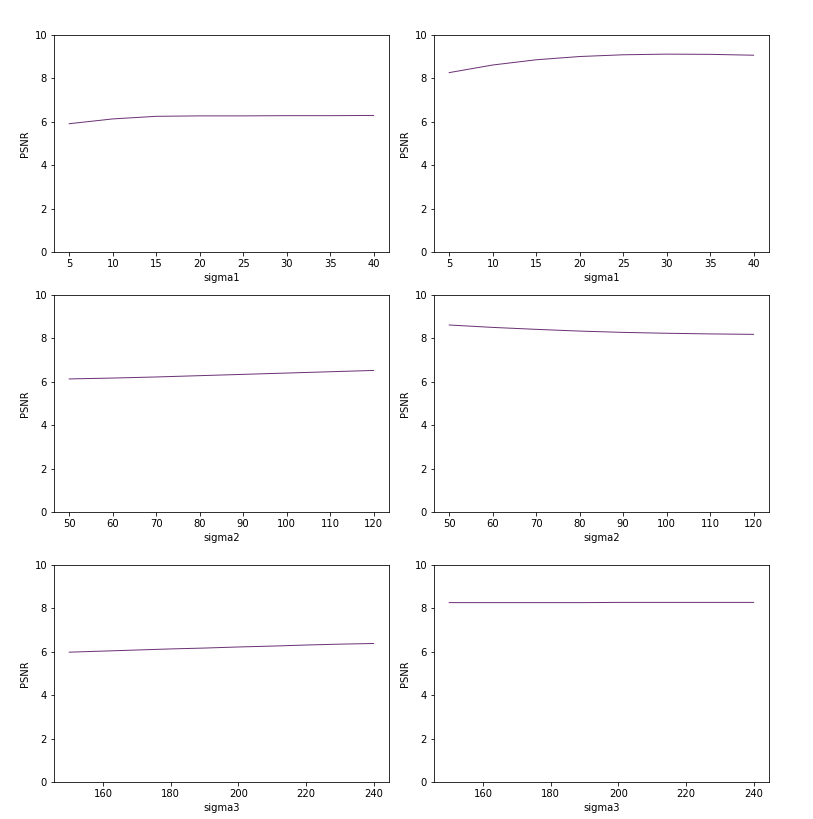
\includegraphics[width=0.7\linewidth]{sn}
	\caption{Variasi Sigma Terhadap Nilai PSNR}
	\label{fig:sn}
\end{figure}
Peneliti melakukan variasi pengujian nilai parameter sigma 1,sigma 2, sigma 3 pada parameter MSR terhadap citra gelap dan citra sedang. Hasil dari variasi nilai parameter terlihat pada gambar 6.4 untuk nilai psnr dan gambar 6.5 untuk nilai deteksi. Variasi nilai yang diberikan untuk sigma 1 [5:40:5], sigma 2 [50:120:10], sigma 3 [150:240:10]. Hasil yang di dapat cenderung stabil dan tidak memiliki nilai puncak. Pada variasi yang diberikan, selisih nilai PSNR tidak memiliki peningkatan yang signifikan dan nilai deteksi cenderung stabil diatas nilai 80. Nilai PSNR citra 1 pada variasi yang diberikan dalam kisaran 6 dan citra 2 dalam kisaran 8 hingga 9,5.
Pada variasi yang diberikan, sigma 1 memiliki pengaruh yang besar pada nilai deteksi. Sigma 1 dengan nilai 5 menghasilkan nilai deteksi 80, seiring nilai sigma 1 ditingkatkan nilai deteksi stabil diatas 90.
\begin{figure}[H]
	\centering
	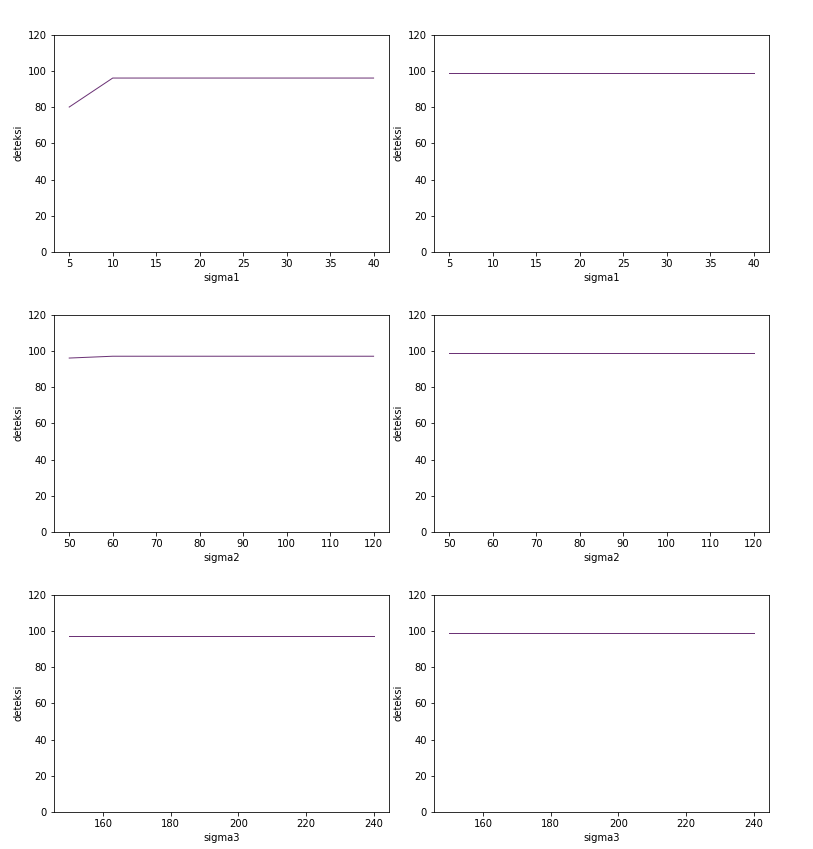
\includegraphics[width=0.8\linewidth]{dtksi}
	\caption{Variasi Sigma Terhadap Nilai Deteksi.}
	\label{fig:dtksi}
\end{figure}

\section{Pengujian Deteksi Tangan}
Pengujuan dilakukan oleh 3 subjek dengan penurunan intensitas cahaya yang sama. Data pada tabel 6.6, 6.7, 6.8, dilakukan oleh subjek pertama, 6.9, 6.10, 6.11, dilakukan oleh subjek kedua, 6.12, 6.13 ,6.14, dilakukan oleh subjek subjek ketiga. Hasil dari ketiga subjek di plot pada grafik gambar 6.6, 6.7, 6.8. 

Kondisi 0 lux  tanpa Retinex pada subjek pertama menghasilkan 40\%, subjek kedua 0\% dan subjek ketiga 50\%, sementara ketika sistem menggunakan Retinex menghasilkan 70\% pada subjek pertama, 70\% pada subjek kedua dan 100\% untuk subjek ketiga. Keadaan pada intensitas 0 lux ini memiliki perbedaan nilai yang sangat jauh, pada citra gelap terlalu susah untuk menemukan dan mengenali objek yang ada. Retinex mampu memberikan perbaikan citra sehingga kontras pada citra meningkat. Peningkatan kontras pada citra dapat membantu sistem mendeteksi keberadaan sebuah objek, terlihat pada gambar 6.6 dan 6.7 menunjukan perubahan sebelum dan sesudah dikenai Retinex.
\begin{figure}[H]
	\centering
	\subfloat[\centering]{{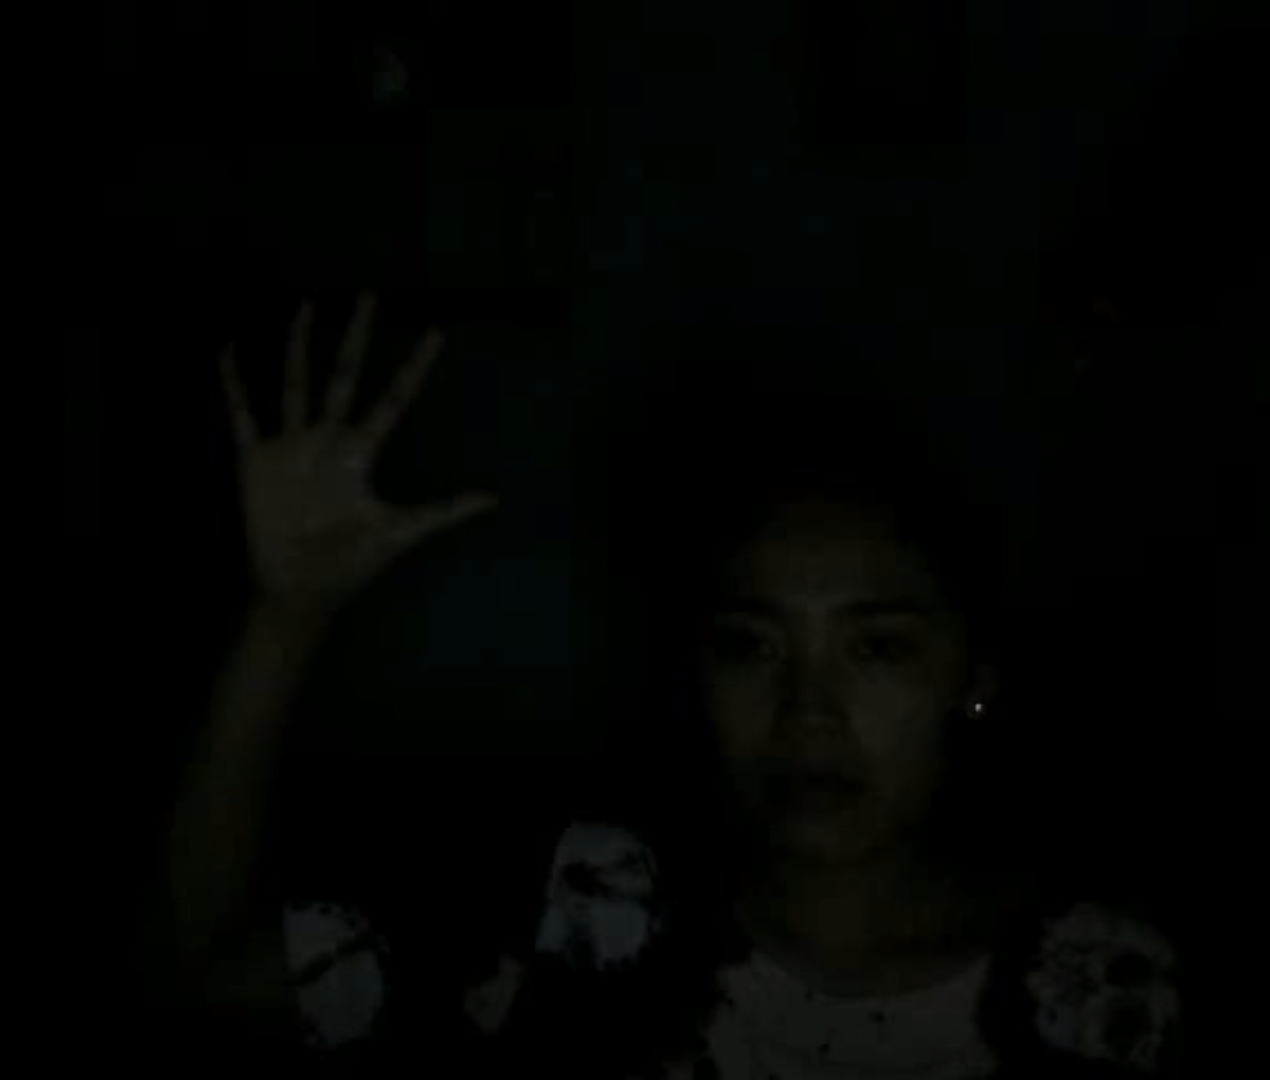
\includegraphics[width=4.84cm]{d} }}%
	\subfloat[\centering]{{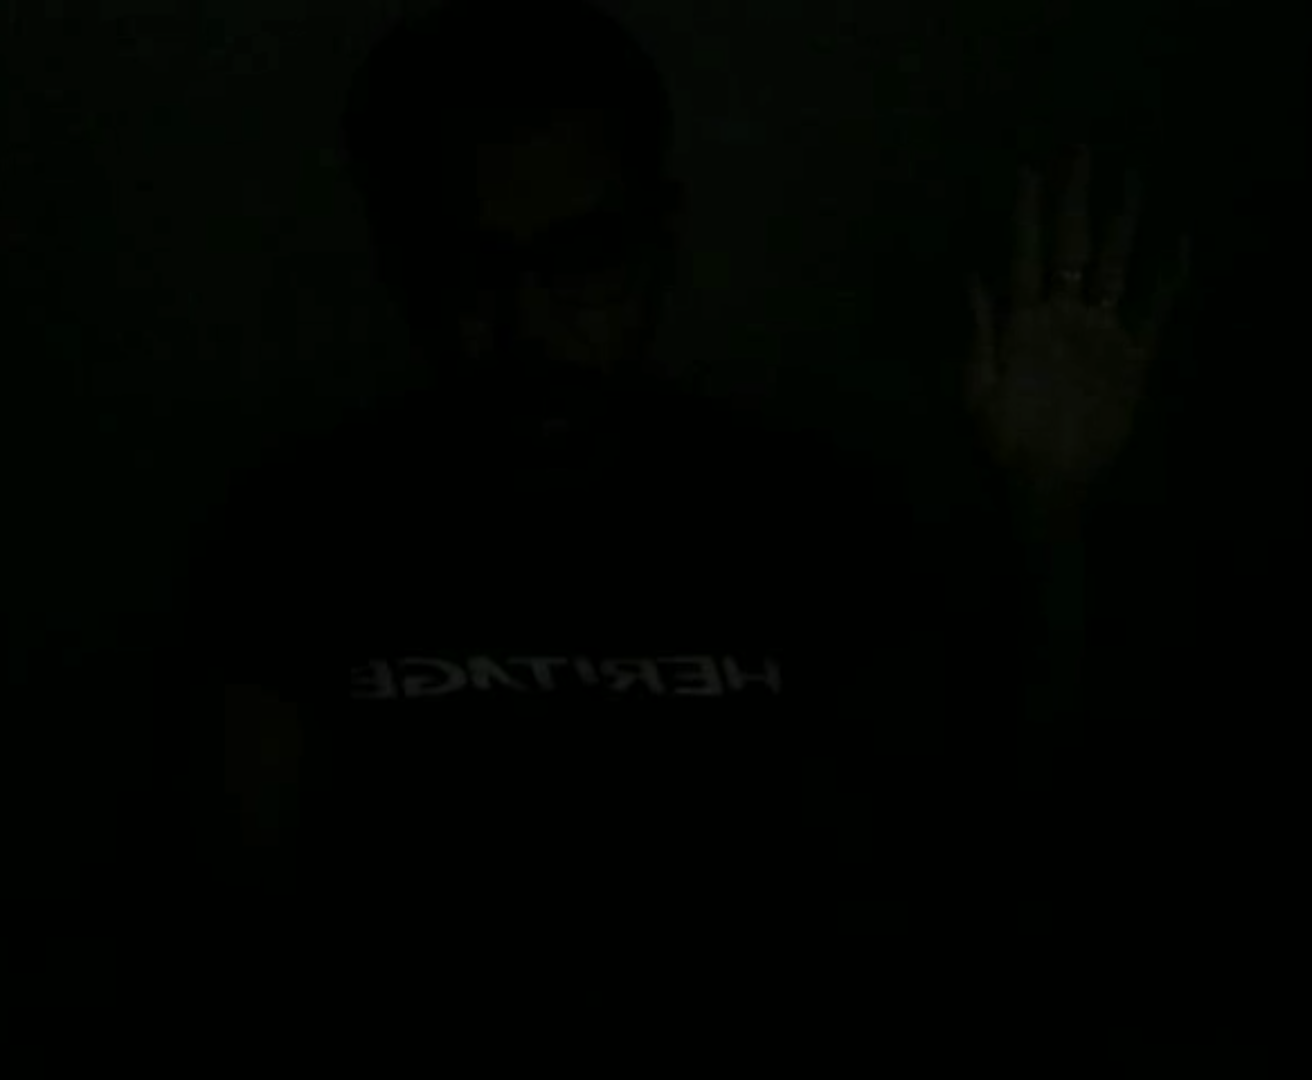
\includegraphics[width=5cm]{saya} }}%
	\caption{Subjek\_1 (a: Subjek 2 tanpa Retinex, b: subjek 3 tanpa Retinex)}
	\quad
	\subfloat[\centering]{{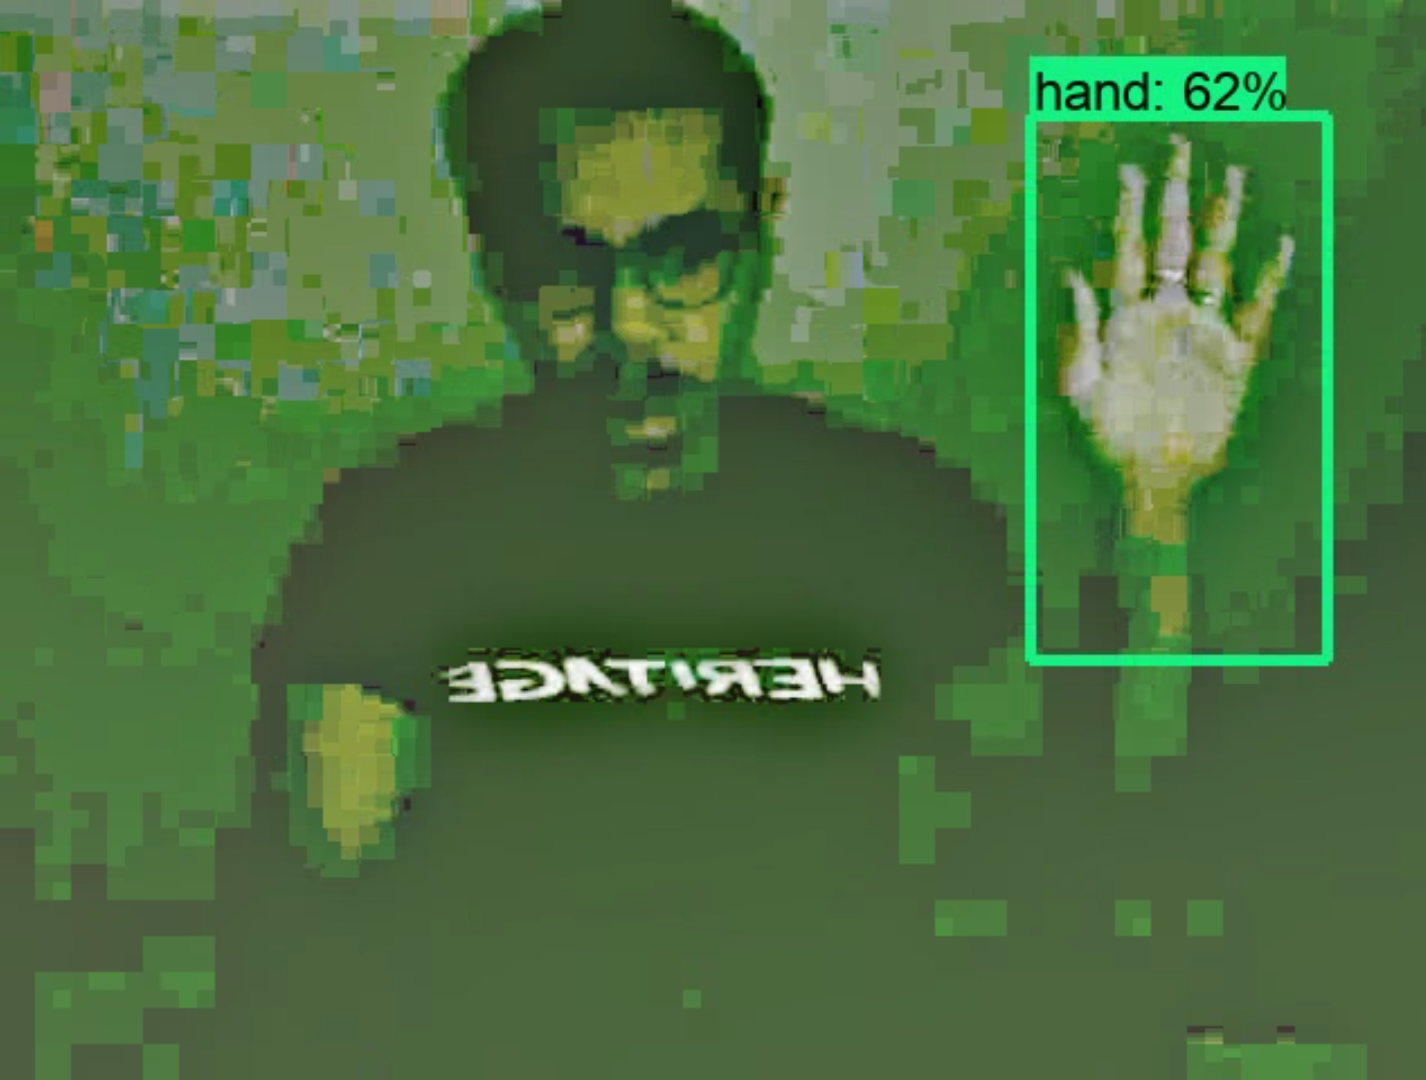
\includegraphics[width=4.8cm]{sayaretinex} }}%
	\subfloat[\centering]{{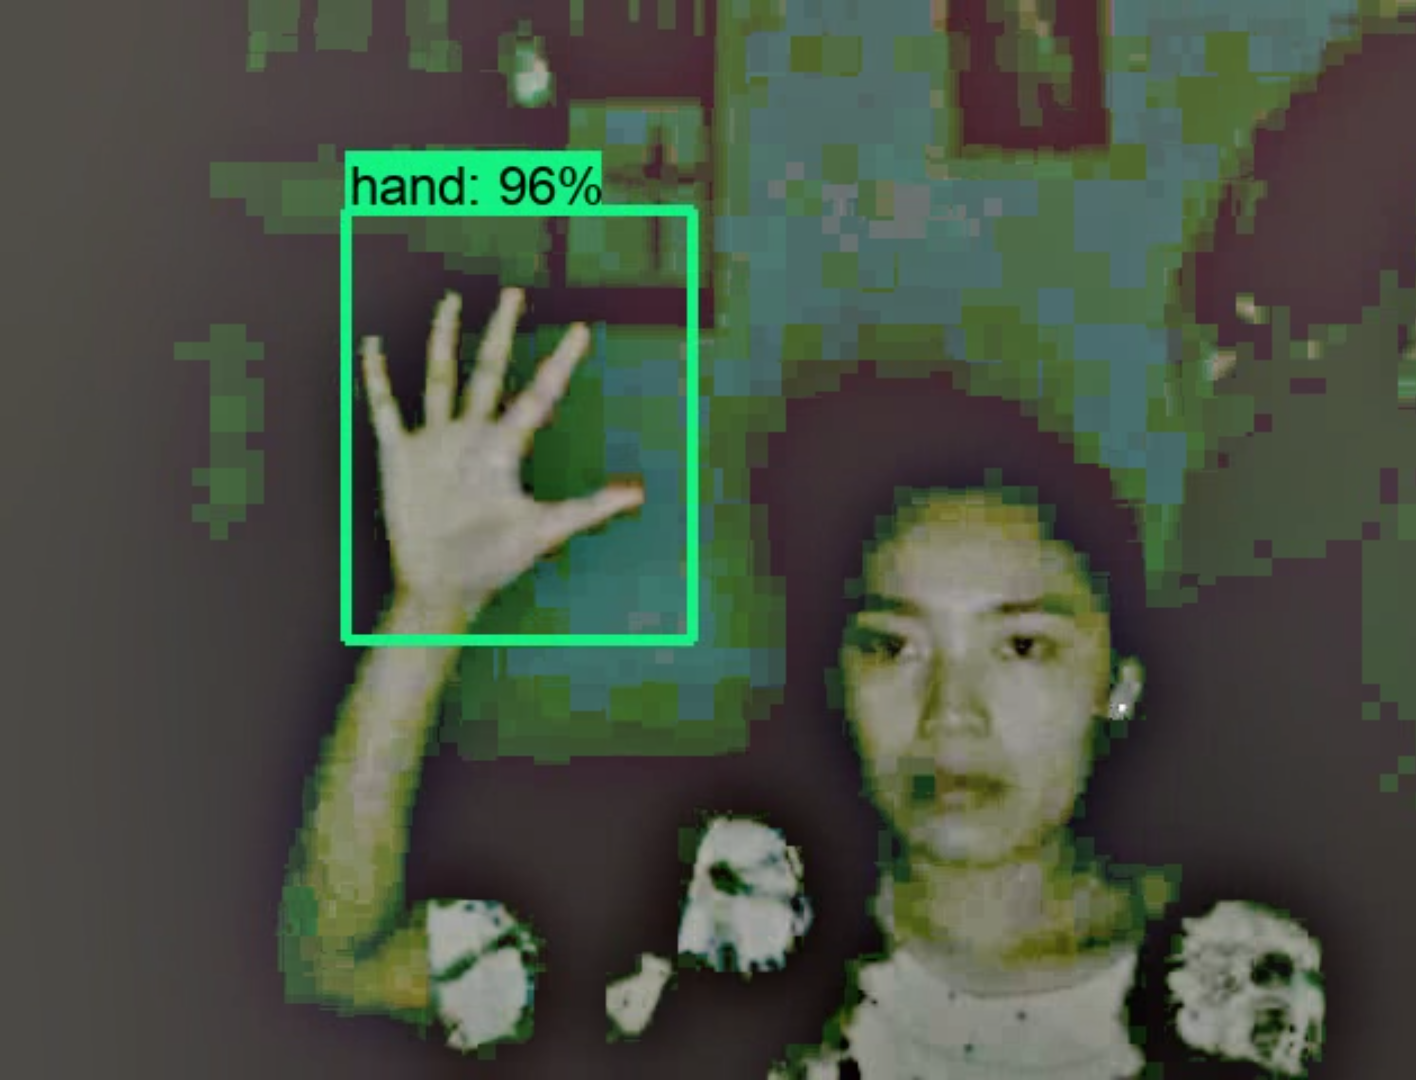
\includegraphics[width=4.8cm]{dretinex} }}%
	\caption{Subjek\_1 (a: Subjek 2 dengan Retinex, b: subjek 3 dengan Retinex)}
	\label{fig:example}%
\end{figure}
Pengujian dengan Retinex menunjukan pada kondisi 0 lux dan 15 lux mendapat nilai 100\%. Pada kondisi intensitas rendah Retinex mampu bekerja dengan baik yang ditunjukan dengan tingkat keberhasilan deteksi. Pengaruh Retinex sangat besar pada kondisi intensitas rendah. Kondisi intensitas diatas 15 lux nilai deteksi yang menggunakan retinex cenderung menurun. Berdasarkan tabel 6.7 pada kondisi intensitas diatas 15 lux sistem masih lebih baik mendeteksi tanpa menggunakan Retinex. Semakin menurun intensitas cahaya sistem tanpa Retinex mengalami penurunan performa yang mengakibatkan tidak mampu mendeteksi objek tangan yang ada, hal ini ditunjukan di grafik perbandingan pada gambar 6.8, 6.9, 6.10.
\begin{table}[H]
	\centering
	\caption{Deteksi Subjek 1 Tanpa Retinex}
	\begin{tabular}{|c|c|c|c|c|c|c|c|c|c|c|}
		\hline Nilai Lux
		& \multicolumn{10}{|c|}{Hasil Deteksi Subjek\_1(Dheo)} \\
		\hline 0 Lux &F &T &F &T &F &T &F &T &F &F\\
		\hline 15 Lux &T &T &T & T&T &T &T &T &T &T\\
		\hline 20 Lux &T &T &T & T&T &T &T &T &T &T\\
		\hline 25 Lux &T &T &T & T&T &T &T &T &T &T\\
		\hline 33 Lux &T &T &T & T&T &T &F &T &T &T\\
		\hline 77 Lux &T &T &T &T &T &T &T &T &T &T\\
		\hline 133 Lux &T &T &T &T &T &T &T &T &F &T\\
		\hline
	\end{tabular}
\end{table}
\begin{table}[H]
	\centering
	\caption{Deteksi Subjek 1 Retinex}
	\begin{tabular}{|c|c|c|c|c|c|c|c|c|c|c|}
		\hline Nilai Lux
		& \multicolumn{10}{|c|}{Hasil Deteksi Subjek\_1(Dheo)} \\
		\hline 0 Lux &F &T &T &T &F &T &T &T &F &T\\
		\hline 15 Lux &T &T &T & T &T &T &T &T &T &T\\
		\hline 20 Lux &T &T &T &T &T &T &T &T &T &T\\
		\hline 25 Lux &T &T &T &T &T &T &T &T &T &T\\
		\hline 33 Lux &T &T &T &T &T &T &T &T &T &T\\
		\hline 77 Lux &T &T &T &T &T &T &T &T &F &T\\
		\hline 133 Lux &F &T &T &F &T &T &T &T &F &T \\
		\hline
	\end{tabular}
\end{table}
\begin{table}[H]
	\caption{Perbandingan Deteksi Tangan Subjek\_1}
	\vspace{0cm}
	\centering
	\begin{tabular}{|c|c|c|}
		\hline Kondisi lux &  Tanpa Retinex &Retinex \\
		\hline  0 lux &40\% &70\% \\
		\hline 15 lux &100\% &100\% \\
		\hline 20 lux &100\% &100\% \\
		\hline 25 lux &100\% &100\% \\
		\hline 33 lux &90\% &100\% \\
		\hline 77 lux &100\% &90\% \\
		\hline 133 lux& 90\% & 70\% \\
		\hline
	\end{tabular}
\end{table}
%%subjek 2
\begin{table}[H]
	\centering
	\caption{Deteksi Subjek 2 Tanpa Retinex}
	\begin{tabular}{|c|c|c|c|c|c|c|c|c|c|c|}
		\hline Nilai Lux
		& \multicolumn{10}{|c|}{Hasil Deteksi Subjek\_2(Saya)} \\
		\hline 0 Lux &F&F&F&F&F&F&F&F&F&F\\
		\hline 15 Lux &T&T&T&T&T&T&T&T&T&T\\
		\hline 20 Lux &T&T&T&T&T&T&T&T&T&T\\
		\hline 25 Lux &T&T&T&T&T&T&T&T&T&T \\
		\hline 33 Lux &T&T&T&T&T&T&T&T&T&T \\
		\hline 77 Lux &T&T&T&T&T&T&T&T&T&T\\
		\hline 133 Lux &T&T&T&T&T&T&T&T&T&T\\
		\hline
	\end{tabular}
\end{table}
\begin{table}[H]
	\centering
	\caption{Deteksi Subjek 2 Retinex}
	\begin{tabular}{|c|c|c|c|c|c|c|c|c|c|c|}
		\hline Nilai Lux
		& \multicolumn{10}{|c|}{Hasil Deteksi Subjek\_2(Saya)} \\
		\hline 0 Lux &T&F&T&F&T&T&F&T&T&T \\
		\hline 15 Lux &T&T&T&T&T&T&T&T&T&T\\
		\hline 20 Lux &F&T&T&F&T&T&T&T&F&T\\
		\hline 25 Lux &T&T&T&T&T&T&F&T&T&T \\
		\hline 33 Lux &T&T&T&T&T&T&T&T&T&T \\
		\hline 77 Lux &T&T&T&T&F&T&F&T&T&T\\
		\hline 133 Lux &T&T&T&T&T&T&T&T&T&T\\
		\hline
	\end{tabular}
\end{table}
\begin{table}[H]
	\caption{Perbandingan Deteksi Tangan Subjek\_2 }
	\vspace{0cm}
	\centering
	\begin{tabular}{|c|c|c|}
		\hline Kondisi lux &  Tanpa Retinex &Retinex \\
		\hline  0 lux& 0\% & 70\% \\
		\hline 15 lux & 100\% &100\% \\
		\hline 20 lux & 100\% &70\% \\
		\hline 25 lux & 100\% &90\% \\
		\hline 33 lux & 100\% &100\% \\
		\hline 77 lux & 100\% &80\% \\
		\hline 133 lux & 100\% &100\%\\
		\hline
	\end{tabular}
\end{table}
%%subjek 3
\begin{table}[H]
	\centering
	\caption{Deteksi Subjek 3 Tanpa Retinex}
	\begin{tabular}{|c|c|c|c|c|c|c|c|c|c|c|}
		\hline Nilai Lux
		& \multicolumn{10}{|c|}{Hasil Deteksi Subjek\_1(Dela)} \\
		\hline 0 Lux &F &T &F &F &T &F &T &T &F &T\\
		\hline 15 Lux &T &T &T &T &T &T &F &F &T &T\\
		\hline 20 Lux &T &T &T &T &T &T &T &T &T &T\\
		\hline 25 Lux &T &T &T &T &T &T &T &T &T &T\\
		\hline 33 Lux &T &T &T &T &T &T &T &T &T &T\\
		\hline 77 Lux &T &T &T &T &T &T &T &T &T &T\\
		\hline 133 Lux &T &T &T &T &T &F &T &T &T &T\\
		\hline
	\end{tabular}
\end{table}
\begin{table}[H]
	\centering
	\caption{Deteksi Subjek 3 Retinex}
	\begin{tabular}{|c|c|c|c|c|c|c|c|c|c|c|}
		\hline Nilai Lux
		& \multicolumn{10}{|c|}{Hasil Deteksi Subjek\_1(Dela)} \\
		\hline 0 Lux &T &T &T &T &T &T &T &T &T &T\\
		\hline 15 Lux &T &T &T &T &T &T &T &T &T &T\\
		\hline 20 Lux  &T &T &T &T &T &T &F &T &T &T\\
		\hline 25 Lux &T &T &T &T &T &T &F &T &T &T\\
		\hline 33 Lux &T &T &F &T &T &T &T &T &T &T\\
		\hline 77 Lux &T &T &T &T &T &T &T &T &T &T\\
		\hline 133 Lux &T &T &T &F &T &T &F &F &T &T\\
		\hline
	\end{tabular}
\end{table}
\begin{table}[H]
	\caption{Perbandingan Deteksi Tangan Subjek\_3 }
	\vspace{0cm}
	\centering
	\begin{tabular}{|c|c|c|}
		\hline Kondisi lux &  Tanpa Retinex &Retinex \\
		\hline  0 lux &50\% &100\%\\
		\hline 15 lux &80\% &100\% \\
		\hline 20 lux &100\% &90\% \\
		\hline 25 lux &100\% &90\% \\
		\hline 33 lux &100\% &90\% \\
		\hline 77 lux &100\% &100\% \\
		\hline 133 lux& 90\% & 70\% \\
		\hline
	\end{tabular}
\end{table}
\begin{figure}[H]
	\centering
	\subfloat[\centering]{{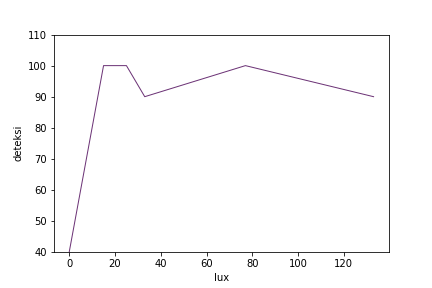
\includegraphics[width=6cm]{OD_dheo} }}%
	\subfloat[\centering]{{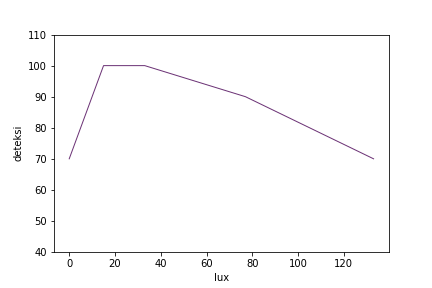
\includegraphics[width=6cm]{msr_OD_dheo} }}%
	\caption{Subjek\_1 (a: Grafik tanpa Retinex, b: Grafik dengan Retinex)}
	\quad
	\subfloat[\centering]{{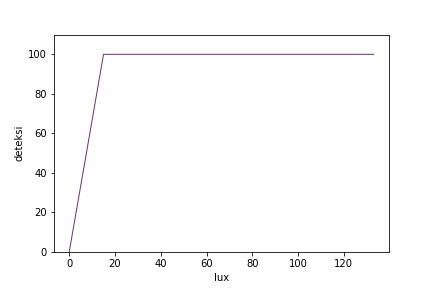
\includegraphics[width=6cm]{OD_saya} }}%
	\subfloat[\centering]{{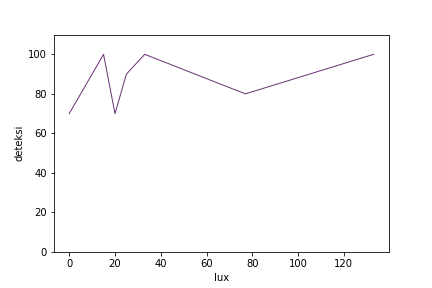
\includegraphics[width=6cm]{msr_OD_saya} }}%
	\caption{Subjek\_2 (a: Grafik tanpa Retinex, b: Grafik dengan Retinex)}
	\quad
	\subfloat[\centering]{{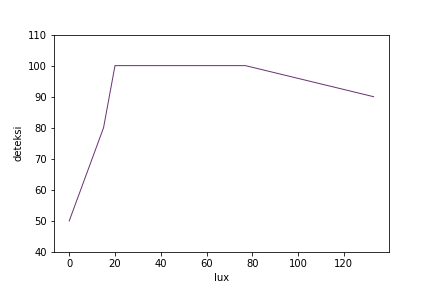
\includegraphics[width=6cm]{OD_dela} }}%
	\subfloat[\centering]{{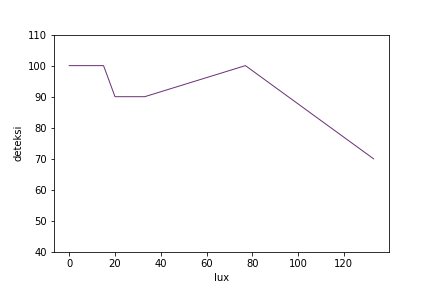
\includegraphics[width=6cm]{msr_OD_dela} }}%
	\caption{Subjek\_3 (a:Grafik tanpa Retinex, b: Grafik dengan Retinex)}%
	\label{fig:example}%
\end{figure}
%Pengujian subjek 3 telah dilakukan perbandingan antara deteksi objek menggunakan retinex dan tanpa retinex, tabel perbandingan ditunjukan pada tabel 6.14. Video tanpa retinex memperoleh nilai deteksi diatas 90\% pada kondisi diatas 15 lux. Penurunan tingkat deteksi sebesar 20\% terjadi pada kondisi 15 lux dan pada kondisi 0 lux sistem hanya mendapatkan nilai 50\%. Semakin menurun intensitas cahaya sistem tanpa Retinex mengalami penurunan performa yang mengakibatkan tidak mampu mendeteksi objek tangan yang ada. Grafik pada pengujian ini ditunjukan pada gambar 6.8.

Berdasarkan ketiga percobaan pengaruh Retinex terlihat pada kondisi lux kurang dari sama dengan 15 lux. Pemberian Retinex pada intensitas yang tinggi menyebabkan \textit{false positive} pada deteksi. Hal tersebut terjadi pada beberapa data dengan intensitas tinggi. Terlihat pada gambar 6.11, semakin terang kondisi cahaya jika diberikan Retinex menyebabkan nilai piksel yang sudah terang akan semakin terang sehingga piksel tersebut dapat berubah nilai menyebabkan objek yang bukan tangan dikenali sebagai tangan. \textit{False positive} sering muncul pada kondisi intensitas diatas 33 lux.
\begin{figure}[H]
	\centering
	\subfloat[\centering]{{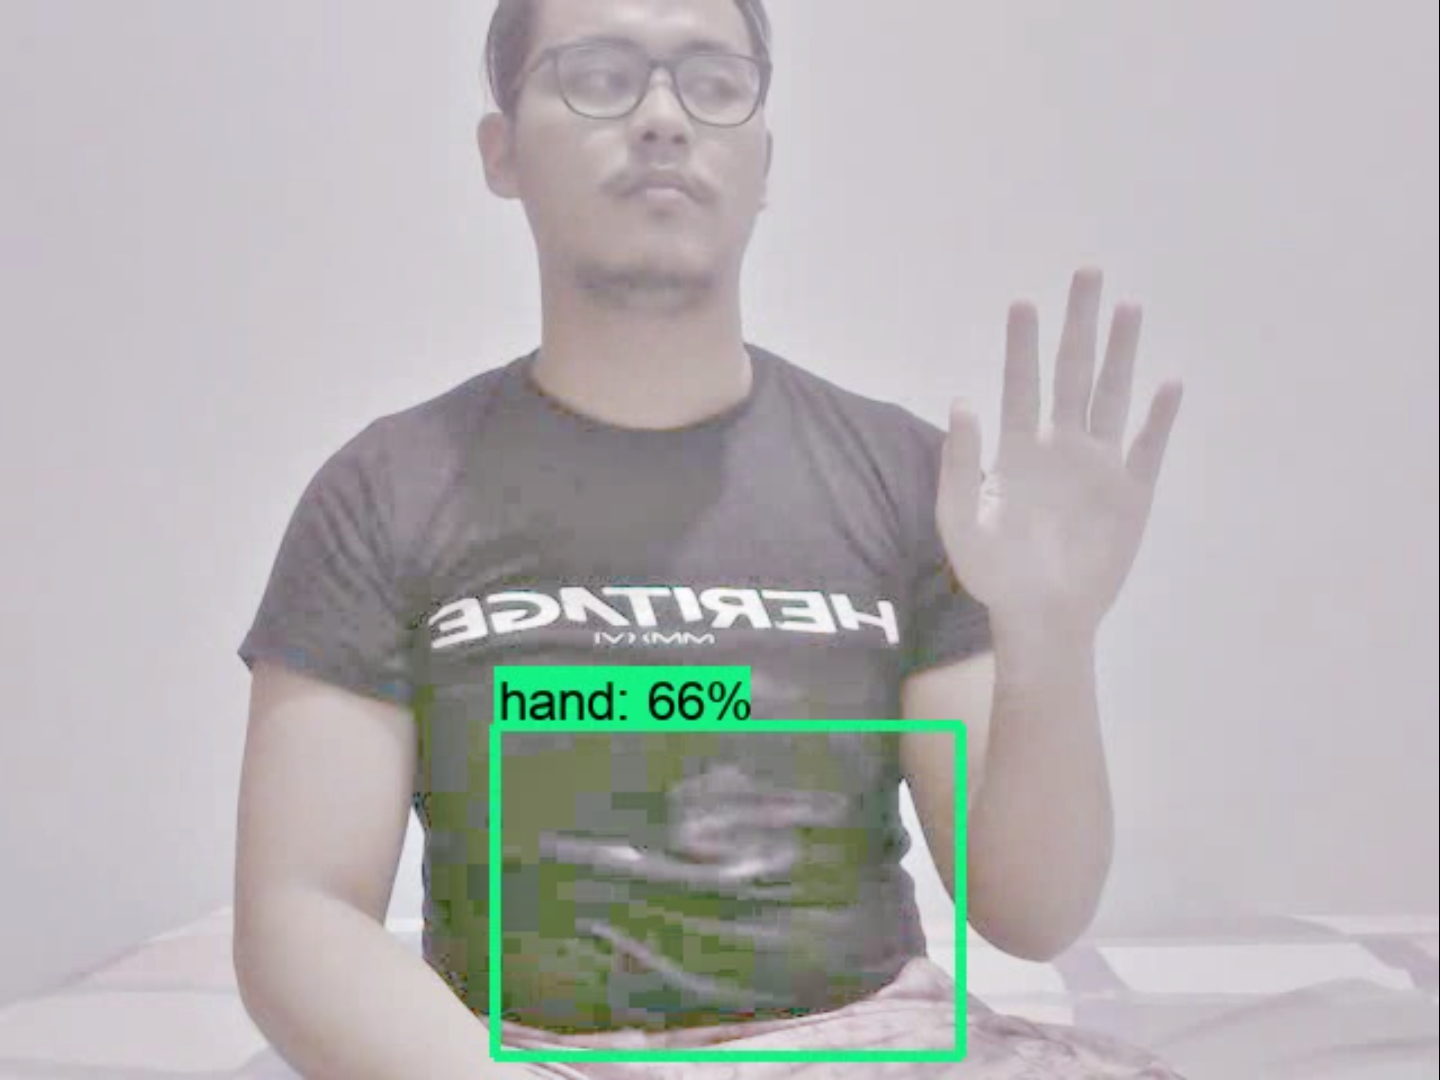
\includegraphics[width=5cm]{FP133} }}%
	\subfloat[\centering]{{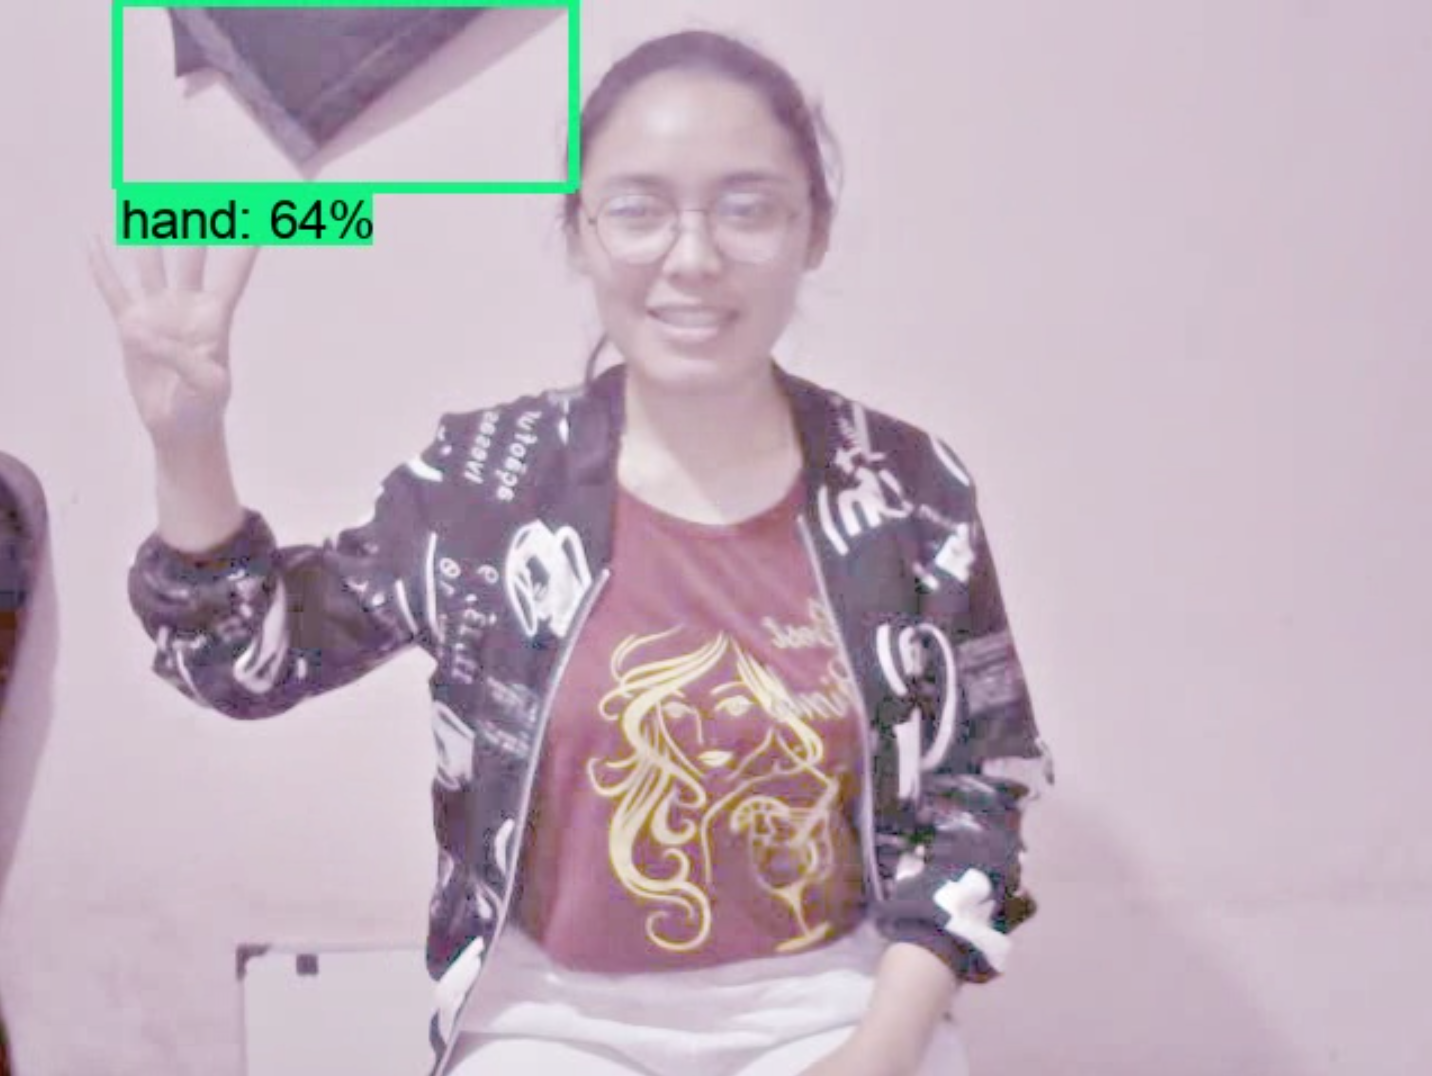
\includegraphics[width=5cm]{FP77} }}%
	\quad
	\subfloat[\centering]{{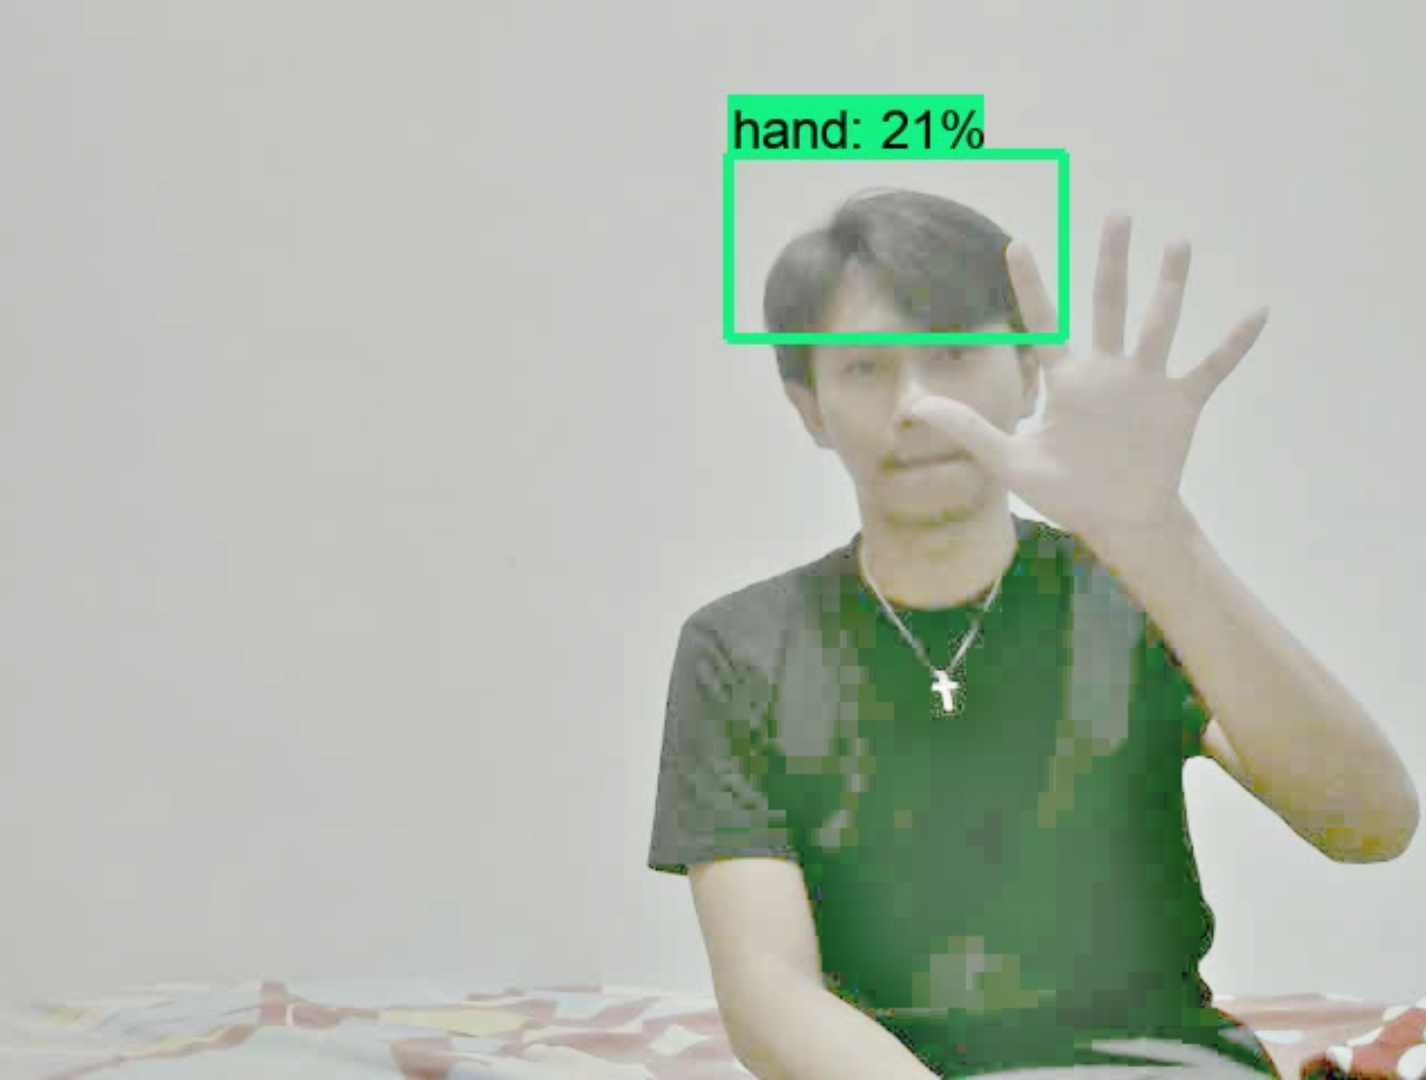
\includegraphics[width=5cm]{FPdeo} }}%
	\caption{Subjek\_1 (a: Kondisi 133 lux, b: Kondisi 77 lux, c:Kondisi 133 lux)}
	\label{fig:example}%
\end{figure}
% TODO: \usepackage{graphicx} required
\section{Pengujian Pengenalan Gestur Tangan}
\begin{tabular}{|c|c|c|c|c|c|c|c|c|c|c|}
	\hline 0 lux
	& \multicolumn{10}{|c|}{Pengenalan Subjek\_1(dheo)} \\
	\hline  Klasifikasi&\textbf{0} &\textbf{1} &\textbf{2} &\textbf{3} &\textbf{4}&\textbf{5} &\textbf{6}&\textbf{7}&\textbf{0}&\textbf{9}\\
	\hline \textbf{Angka 0} &\textbf{0} &0 &0 &0 &0 &0 &0 &0 &0 &0\\
	\hline \textbf{Angka 1} &0 &\textbf{0} &0 &0 &0 &0 &0 &0 &0 &0\\
	\hline \textbf{Angka 2} &0 &0 &\textbf{0} &0 &0 &0 &0 &0 &0 &0\\
	\hline \textbf{Angka 3} &0 &0 &0 &\textbf{0} &0 &0 &0 &0 &0 &0\\
	\hline \textbf{Angka 4} &0 &0 &0 &0 &\textbf{0} &0 &0 &0 &0 &0\\
	\hline \textbf{Angka 5} &0 &0 &0 &0 &0 &\textbf{0} &0 &0 &0 &0\\
	\hline \textbf{Angka 6} &0 &0 &0 &0 &0 &0 &\textbf{0} &0 &0 &0\\
	\hline \textbf{Angka 7} &0 &0 &0 &0 &0 &0 &0 &\textbf{0} &0 &0\\
	\hline \textbf{Angka 8} &0 &0 &0 &0 &0 &0 &0 &0 &\textbf{0} &0 \\
	\hline \textbf{Angka 9} &0 &0 &0 &0 &0 &0 &0 &0 &0 &\textbf{0} \\
	\hline
\end{tabular}

\begin{tabular}{|c|c|c|c|c|c|c|c|c|c|c|}
	\hline 15 lux
	& \multicolumn{10}{|c|}{Pengenalan Subjek\_1(dheo)} \\
	\hline  Klasifikasi&\textbf{0} &\textbf{1} &\textbf{2} &\textbf{3} &\textbf{4}&\textbf{5} &\textbf{6}&\textbf{7}&\textbf{8}&\textbf{9}\\
	\hline \textbf{Angka 0} &\textbf{10} &0 &0 &0 &0 &0 &0 &0 &0 &0\\
	\hline \textbf{Angka 1} &0 &\textbf{10} &0 &0 &0 &0 &0 &0 &0 &0\\
	\hline \textbf{Angka 2} &0 &0 &\textbf{9} &\textbf{1} &0 &0 &0 &0 &0 &0\\
	\hline \textbf{Angka 3} &0 &0 &0 &\textbf{10} &0 &0 &0 &0 &0 &0\\
	\hline \textbf{Angka 4} &0 &0 &0 &0 &\textbf{9} &0 &0 &0 &0 &\textbf{1}\\
	\hline \textbf{Angka 5} &0 &0 &0 &0 &0 &\textbf{10} &0 &0 &0 &0\\
	\hline \textbf{Angka 6} &0 &0 &0 &0 &0 &0 &\textbf{10} &0 &0 &0\\
	\hline \textbf{Angka 7} &0 &0 &0 &\textbf{2} &\textbf{1} &0 &0 &\textbf{4} &\textbf{2} &\textbf{1}\\
	\hline \textbf{Angka 8} &0 &0 &0 &0 &0 &0 &0 &0 &\textbf{8} &\textbf{2} \\
	\hline \textbf{Angka 9} &0 &0 &0 &0 &0 &0 &0 &0 &0 &\textbf{10} \\
	\hline
\end{tabular}

\begin{tabular}{|c|c|c|c|c|c|c|c|c|c|c|}
	\hline 20 lux
	& \multicolumn{10}{|c|}{Pengenalan Subjek\_1(dheo)} \\
	\hline  Klasifikasi&\textbf{0} &\textbf{1} &\textbf{2} &\textbf{3} &\textbf{4}&\textbf{5} &\textbf{6}&\textbf{7}&\textbf{0}&\textbf{9}\\
	\hline \textbf{Angka 0} &\textbf{0} &0 &0 &0 &0 &0 &0 &0 &0 &0\\
	\hline \textbf{Angka 1} &0 &\textbf{0} &0 &0 &0 &0 &0 &0 &0 &0\\
	\hline \textbf{Angka 2} &0 &0 &\textbf{0} &\textbf{1} &0 &0 &0 &0 &0 &0\\
	\hline \textbf{Angka 3} &0 &0 &0 &\textbf{0} &0 &0 &0 &0 &0 &0\\
	\hline \textbf{Angka 4} &0 &0 &0 &0 &\textbf{0} &0 &0 &0 &0 &\textbf{1}\\
	\hline \textbf{Angka 5} &0 &0 &0 &0 &0 &\textbf{00} &0 &0 &0 &0\\
	\hline \textbf{Angka 6} &0 &0 &0 &0 &0 &0 &\textbf{0} &0 &0 &0\\
	\hline \textbf{Angka 7} &0 &0 &0 &\textbf{2} &\textbf{0} &0 &0 &\textbf{4} &\textbf{2} &\textbf{1}\\
	\hline \textbf{Angka 8} &0 &0 &0 &0 &0 &0 &0 &0 &\textbf{0} &\textbf{2} \\
	\hline \textbf{Angka 9} &0 &0 &0 &0 &0 &0 &0 &0 &0 &\textbf{0} \\
	\hline
\end{tabular}

\begin{tabular}{|c|c|c|c|c|c|c|c|c|c|c|}
	\hline 25 lux
	& \multicolumn{10}{|c|}{Pengenalan Subjek\_1(dheo)} \\
	\hline  Klasifikasi&\textbf{0} &\textbf{1} &\textbf{2} &\textbf{3} &\textbf{4}&\textbf{5} &\textbf{6}&\textbf{7}&\textbf{0}&\textbf{9}\\
	\hline \textbf{Angka 0} &\textbf{0} &0 &0 &0 &0 &0 &0 &0 &0 &0\\
	\hline \textbf{Angka 1} &0 &\textbf{0} &0 &0 &0 &0 &0 &0 &0 &0\\
	\hline \textbf{Angka 2} &0 &0 &\textbf{0} &\textbf{1} &0 &0 &0 &0 &0 &0\\
	\hline \textbf{Angka 3} &0 &0 &0 &\textbf{0} &0 &0 &0 &0 &0 &0\\
	\hline \textbf{Angka 4} &0 &0 &0 &0 &\textbf{0} &0 &0 &0 &0 &\textbf{1}\\
	\hline \textbf{Angka 5} &0 &0 &0 &0 &0 &\textbf{00} &0 &0 &0 &0\\
	\hline \textbf{Angka 6} &0 &0 &0 &0 &0 &0 &\textbf{0} &0 &0 &0\\
	\hline \textbf{Angka 7} &0 &0 &0 &\textbf{2} &\textbf{0} &0 &0 &\textbf{4} &\textbf{2} &\textbf{1}\\
	\hline \textbf{Angka 8} &0 &0 &0 &0 &0 &0 &0 &0 &\textbf{0} &\textbf{2} \\
	\hline \textbf{Angka 9} &0 &0 &0 &0 &0 &0 &0 &0 &0 &\textbf{0} \\
	\hline
\end{tabular}

\begin{tabular}{|c|c|c|c|c|c|c|c|c|c|c|}
	\hline 33 lux
	& \multicolumn{10}{|c|}{Pengenalan Subjek\_1(dheo)} \\
	\hline  Klasifikasi&\textbf{0} &\textbf{1} &\textbf{2} &\textbf{3} &\textbf{4}&\textbf{5} &\textbf{6}&\textbf{7}&\textbf{8}&\textbf{9}\\
	\hline \textbf{Angka 0} &\textbf{10} &0 &0 &0 &0 &0 &0 &0 &0 &0\\
	\hline \textbf{Angka 1} &0 &\textbf{9} &\textbf{1} &0 &0 &0 &0 &0 &0 &0\\
	\hline \textbf{Angka 2} &0 &0 &\textbf{10} &0 &0 &0 &0 &0 &0 &0\\
	\hline \textbf{Angka 3} &0 &0 &0 &\textbf{10} &0 &0 &0 &0 &0 &0\\
	\hline \textbf{Angka 4} &0 &0 &0 &0 &\textbf{10} &0 &0 &0 &0 &0\\
	\hline \textbf{Angka 5} &0 &0 &0 &0 &0 &\textbf{10} &0 &0 &0 &0\\
	\hline \textbf{Angka 6} &0 &0 &0 &0 &0 &0 &\textbf{10} &0 &0 &0\\
	\hline \textbf{Angka 7} &0 &0 &0 &0 &0 &0 &0 &\textbf{10} &0 &0\\
	\hline \textbf{Angka 8} &0 &0 &0 &0 &0 &0 &0 &0 &\textbf{9} &\textbf{1} \\
	\hline \textbf{Angka 9} &0 &0 &0 &0 &0 &0 &0 &0 &0 &\textbf{10} \\
	\hline
\end{tabular}

\begin{tabular}{|c|c|c|c|c|c|c|c|c|c|c|}
	\hline 77 lux
	& \multicolumn{10}{|c|}{Pengenalan Subjek\_1(dheo)} \\
	\hline  Klasifikasi&\textbf{0} &\textbf{1} &\textbf{2} &\textbf{3} &\textbf{4}&\textbf{5} &\textbf{6}&\textbf{7}&\textbf{8}&\textbf{9}\\
	\hline \textbf{Angka 0} &\textbf{10} &0 &0 &0 &0 &0 &0 &0 &0 &0\\
	\hline \textbf{Angka 1} &0 &\textbf{10} &0 &0 &0 &0 &0 &0 &0 &0\\
	\hline \textbf{Angka 2} &0 &0 &\textbf{10} &0 &0 &0 &0 &0 &0 &0\\
	\hline \textbf{Angka 3} &0 &0 &0 &\textbf{10} &0 &0 &0 &0 &0 &0\\
	\hline \textbf{Angka 4} &0 &0 &0 &0 &\textbf{10} &0 &0 &0 &0 &0\\
	\hline \textbf{Angka 5} &0 &0 &0 &0 &0 &\textbf{10} &0 &0 &0 &0\\
	\hline \textbf{Angka 6} &0 &0 &0 &0 &0 &0 &\textbf{10} &0 &0 &0\\
	\hline \textbf{Angka 7} &0 &0 &0 &0 &0 &0 &0 &\textbf{10} &0 &0\\
	\hline \textbf{Angka 8} &0 &0 &0 &0 &0 &0 &0 &0 &\textbf{10} &0 \\
	\hline \textbf{Angka 9} &0 &0 &0 &0 &0 &0 &0 &0 &0 &\textbf{10} \\
	\hline
\end{tabular}

\begin{tabular}{|c|c|c|c|c|c|c|c|c|c|c|}
	\hline 133 lux
	& \multicolumn{10}{|c|}{Pengenalan Subjek\_1(dheo)} \\
	\hline  Klasifikasi&\textbf{0} &\textbf{1} &\textbf{2} &\textbf{3} &\textbf{4}&\textbf{5} &\textbf{6}&\textbf{7}&\textbf{8}&\textbf{9}\\
	\hline \textbf{Angka 0} &\textbf{10} &0 &0 &0 &0 &0 &0 &0 &0 &0\\
	\hline \textbf{Angka 1} &0 &\textbf{10} &0 &0 &0 &0 &0 &0 &0 &0\\
	\hline \textbf{Angka 2} &0 &0 &\textbf{10} &0 &0 &0 &0 &0 &0 &0\\
	\hline \textbf{Angka 3} &0 &0 &0 &\textbf{10} &0 &0 &0 &0 &0 &0\\
	\hline \textbf{Angka 4} &0 &0 &0 &0 &\textbf{10} &0 &0 &0 &0 &0\\
	\hline \textbf{Angka 5} &0 &0 &0 &0 &0 &\textbf{10} &0 &0 &0 &0\\
	\hline \textbf{Angka 6} &0 &0 &0 &0 &0 &0 &\textbf{10} &0 &0 &0\\
	\hline \textbf{Angka 7} &0 &0 &0 &0 &0 &0 &0 &\textbf{10} &0 &0\\
	\hline \textbf{Angka 8} &0 &0 &0 &0 &0 &0 &0 &0 &\textbf{10} &0 \\
	\hline \textbf{Angka 9} &0 &0 &0 &0 &0 &0 &0 &0 &0 &\textbf{10} \\
	\hline
\end{tabular}

WITH RETINEX

\begin{tabular}{|c|c|c|c|c|c|c|c|c|c|c|}
	\hline 0 lux
	& \multicolumn{10}{|c|}{Pengenalan Subjek\_1(dheo)} \\
	\hline  Klasifikasi&\textbf{0} &\textbf{1} &\textbf{2} &\textbf{3} &\textbf{4}&\textbf{5} &\textbf{6}&\textbf{7}&\textbf{0}&\textbf{9}\\
	\hline \textbf{Angka 0} &\textbf{0} &0 &0 &0 &0 &0 &0 &0 &0 &0\\
	\hline \textbf{Angka 1} &0 &\textbf{0} &0 &0 &0 &0 &0 &0 &0 &0\\
	\hline \textbf{Angka 2} &0 &0 &\textbf{0} &0 &0 &0 &0 &0 &0 &0\\
	\hline \textbf{Angka 3} &0 &0 &0 &\textbf{0} &0 &0 &0 &0 &0 &0\\
	\hline \textbf{Angka 4} &0 &0 &0 &0 &\textbf{0} &0 &0 &0 &0 &0\\
	\hline \textbf{Angka 5} &0 &0 &0 &0 &0 &\textbf{0} &0 &0 &0 &0\\
	\hline \textbf{Angka 6} &0 &0 &0 &0 &0 &0 &\textbf{0} &0 &0 &0\\
	\hline \textbf{Angka 7} &0 &0 &0 &0 &0 &0 &0 &\textbf{0} &0 &0\\
	\hline \textbf{Angka 8} &0 &0 &0 &0 &0 &0 &0 &0 &\textbf{0} &0 \\
	\hline \textbf{Angka 9} &0 &0 &0 &0 &0 &0 &0 &0 &0 &\textbf{0} \\
	\hline
\end{tabular}

\begin{tabular}{|c|c|c|c|c|c|c|c|c|c|c|}
	\hline 15 lux
	& \multicolumn{10}{|c|}{Pengenalan Subjek\_1(dheo)} \\
	\hline  Klasifikasi&\textbf{0} &\textbf{1} &\textbf{2} &\textbf{3} &\textbf{4}&\textbf{5} &\textbf{6}&\textbf{7}&\textbf{8}&\textbf{9}\\
	\hline \textbf{Angka 0} &\textbf{10} &0 &0 &0 &0 &0 &0 &0 &0 &0\\
	\hline \textbf{Angka 1} &0 &\textbf{8} &\textbf{2} &0 &0 &0 &0 &0 &0 &0\\
	\hline \textbf{Angka 2} &0 &0 &\textbf{10} &0 &0 &0 &0 &0 &0 &0\\
	\hline \textbf{Angka 3} &0 &0 &\textbf{2} &\textbf{7} &\textbf{1} &0 &0 &0 &0 &0\\
	\hline \textbf{Angka 4} &0 &0 &0 &0 &\textbf{7} &0 &\textbf{3} &0 &0 &\textbf{1}\\
	\hline \textbf{Angka 5} &0 &0 &0 &0 &\textbf{10} &0 &0 &0 &0 &0\\
	\hline \textbf{Angka 6} &0 &0 &0 &0 &0 &0 &\textbf{10} &0 &0 &0\\
	\hline \textbf{Angka 7} &0 &0 &\textbf{2} &0 &0 &0 &\textbf{6} &\textbf{2} &0 &0\\
	\hline \textbf{Angka 8} &0 &0 &\textbf{2} &0 &0 &0 &0 &\textbf{7} &\textbf{1} &0 \\
	\hline \textbf{Angka 9} &0 &0 &\textbf{3} &\textbf{2} &\textbf{1} &0 &\textbf{4} &0 &0 &\textbf{0} \\
	\hline
\end{tabular}

\begin{tabular}{|c|c|c|c|c|c|c|c|c|c|c|}
	\hline 20 lux
	& \multicolumn{10}{|c|}{Pengenalan Subjek\_1(dheo)} \\
	\hline  Klasifikasi&\textbf{0} &\textbf{1} &\textbf{2} &\textbf{3} &\textbf{4}&\textbf{5} &\textbf{6}&\textbf{7}&\textbf{0}&\textbf{9}\\
	\hline \textbf{Angka 0} &\textbf{0} &0 &0 &0 &0 &0 &0 &0 &0 &0\\
	\hline \textbf{Angka 1} &0 &\textbf{0} &0 &0 &0 &0 &0 &0 &0 &0\\
	\hline \textbf{Angka 2} &0 &0 &\textbf{0} &\textbf{1} &0 &0 &0 &0 &0 &0\\
	\hline \textbf{Angka 3} &0 &0 &0 &\textbf{0} &0 &0 &0 &0 &0 &0\\
	\hline \textbf{Angka 4} &0 &0 &0 &0 &\textbf{0} &0 &0 &0 &0 &\textbf{1}\\
	\hline \textbf{Angka 5} &0 &0 &0 &0 &0 &\textbf{00} &0 &0 &0 &0\\
	\hline \textbf{Angka 6} &0 &0 &0 &0 &0 &0 &\textbf{0} &0 &0 &0\\
	\hline \textbf{Angka 7} &0 &0 &0 &\textbf{2} &\textbf{0} &0 &0 &\textbf{4} &\textbf{2} &\textbf{1}\\
	\hline \textbf{Angka 8} &0 &0 &0 &0 &0 &0 &0 &0 &\textbf{0} &\textbf{2} \\
	\hline \textbf{Angka 9} &0 &0 &0 &0 &0 &0 &0 &0 &0 &\textbf{0} \\
	\hline
\end{tabular}

\begin{tabular}{|c|c|c|c|c|c|c|c|c|c|c|}
	\hline 25 lux
	& \multicolumn{10}{|c|}{Pengenalan Subjek\_1(dheo)} \\
	\hline  Klasifikasi&\textbf{0} &\textbf{1} &\textbf{2} &\textbf{3} &\textbf{4}&\textbf{5} &\textbf{6}&\textbf{7}&\textbf{0}&\textbf{9}\\
	\hline \textbf{Angka 0} &\textbf{0} &0 &0 &0 &0 &0 &0 &0 &0 &0\\
	\hline \textbf{Angka 1} &0 &\textbf{0} &0 &0 &0 &0 &0 &0 &0 &0\\
	\hline \textbf{Angka 2} &0 &0 &\textbf{0} &\textbf{1} &0 &0 &0 &0 &0 &0\\
	\hline \textbf{Angka 3} &0 &0 &0 &\textbf{0} &0 &0 &0 &0 &0 &0\\
	\hline \textbf{Angka 4} &0 &0 &0 &0 &\textbf{0} &0 &0 &0 &0 &\textbf{1}\\
	\hline \textbf{Angka 5} &0 &0 &0 &0 &0 &\textbf{0} &0 &0 &0 &0\\
	\hline \textbf{Angka 6} &0 &0 &0 &0 &0 &0 &\textbf{0} &0 &0 &0\\
	\hline \textbf{Angka 7} &0 &0 &0 &\textbf{2} &\textbf{0} &0 &0 &\textbf{4} &\textbf{2} &\textbf{1}\\
	\hline \textbf{Angka 8} &0 &0 &0 &0 &0 &0 &0 &0 &\textbf{0} &\textbf{2} \\
	\hline \textbf{Angka 9} &0 &0 &0 &0 &0 &0 &0 &0 &0 &\textbf{0} \\
	\hline
\end{tabular}

\begin{tabular}{|c|c|c|c|c|c|c|c|c|c|c|}
	\hline 33 lux
	& \multicolumn{10}{|c|}{Pengenalan Subjek\_1(dheo)} \\
	\hline  Klasifikasi&\textbf{0} &\textbf{1} &\textbf{2} &\textbf{3} &\textbf{4}&\textbf{5} &\textbf{6}&\textbf{7}&\textbf{8}&\textbf{9}\\
	\hline \textbf{Angka 0} &\textbf{10} &0 &0 &0 &0 &0 &0 &0 &0 &0\\
	\hline \textbf{Angka 1} &0 &\textbf{6} &\textbf{4} &0 &0 &0 &0 &0 &0 &0\\
	\hline \textbf{Angka 2} &0 &0 &\textbf{10} &0 &0 &0 &0 &0 &0 &0\\
	\hline \textbf{Angka 3} &0 &0 &0 &\textbf{10} &0 &0 &0 &0 &0 &0\\
	\hline \textbf{Angka 4} &0 &0 &0 &0 &\textbf{5} &\textbf{5} &0 &0 &0 &0\\
	\hline \textbf{Angka 5} &0 &0 &0 &0 &0 &\textbf{10} &0 &0 &0 &0\\
	\hline \textbf{Angka 6} &0 &0 &0 &0 &0 &0 &\textbf{10} &0 &0 &0\\
	\hline \textbf{Angka 7} &0 &0 &\textbf{3} &0 &0 &0 &0 &\textbf{10} &0 &0\\
	\hline \textbf{Angka 8} &0 &0 &\textbf{2} &0 &0 &0 &0 &\textbf{1} &\textbf{7} &0 \\
	\hline \textbf{Angka 9} &0 &0 &\textbf{2} &\textbf{2} &0 &0 &\textbf{6} &0 &0 &\textbf{4} \\
	\hline
\end{tabular}

\begin{tabular}{|c|c|c|c|c|c|c|c|c|c|c|}
	\hline 77 lux
	& \multicolumn{10}{|c|}{Pengenalan Subjek\_1(dheo)} \\
	\hline  Klasifikasi&\textbf{0} &\textbf{1} &\textbf{2} &\textbf{3} &\textbf{4}&\textbf{5} &\textbf{6}&\textbf{7}&\textbf{8}&\textbf{9}\\
	\hline \textbf{Angka 0} &\textbf{10} &0 &0 &0 &0 &0 &0 &0 &0 &0\\
	\hline \textbf{Angka 1} &0 &\textbf{8} &\textbf{2} &0 &0 &0 &0 &0 &0 &0\\
	\hline \textbf{Angka 2} &0 &0 &\textbf{10} &0 &0 &0 &0 &0 &0 &0\\
	\hline \textbf{Angka 3} &0 &0 &0 &\textbf{10} &0 &0 &0 &0 &0 &0\\
	\hline \textbf{Angka 4} &0 &0 &0 &0 &\textbf{5} &0 &\textbf{5} &0 &0 &0\\
	\hline \textbf{Angka 5} &0 &0 &0 &0 &\textbf{1} &\textbf{9} &0 &0 &0 &0\\
	\hline \textbf{Angka 6} &0 &0 &\textbf{1} &0 &0 &0 &\textbf{9} &0 &0 &0\\
	\hline \textbf{Angka 7} &0 &0 &\textbf{2} &0 &0 &0 &0 &\textbf{8} &0 &0\\
	\hline \textbf{Angka 8} &0 &0 &0 &0 &0 &0 &0 &0 &\textbf{10} &0 \\
	\hline \textbf{Angka 9} &0 &0 &\textbf{4} &\textbf{2} &0 &0 &0 &0 &0 &\textbf{4} \\
	\hline
\end{tabular}

\begin{tabular}{|c|c|c|c|c|c|c|c|c|c|c|}
	\hline 133 lux
	& \multicolumn{10}{|c|}{Pengenalan Subjek\_1(dheo)} \\
	\hline  Klasifikasi&\textbf{0} &\textbf{1} &\textbf{2} &\textbf{3} &\textbf{4}&\textbf{5} &\textbf{6}&\textbf{7}&\textbf{8}&\textbf{9}\\
	\hline \textbf{Angka 0} &\textbf{10} &0 &0 &0 &0 &0 &0 &0 &0 &0\\
	\hline \textbf{Angka 1} &0 &\textbf{10} &0 &0 &0 &0 &0 &0 &0 &0\\
	\hline \textbf{Angka 2} &0 &0 &\textbf{10} &0 &0 &0 &0 &0 &0 &0\\
	\hline \textbf{Angka 3} &0 &0 &0 &\textbf{10} &0 &0 &0 &0 &0 &0\\
	\hline \textbf{Angka 4} &0 &0 &0 &0 &\textbf{10} &0 &0 &0 &0 &0\\
	\hline \textbf{Angka 5} &0 &0 &0 &\textbf{1} &\textbf{1} &\textbf{8} &0 &0 &0 &0\\
	\hline \textbf{Angka 6} &0 &0 &0 &0 &0 &0 &\textbf{10} &0 &0 &0\\
	\hline \textbf{Angka 7} &0 &0 &0 &0 &0 &0 &0 &\textbf{10} &0 &0\\
	\hline \textbf{Angka 8} &0 &0 &0 &0 &0 &0 &0 &0 &\textbf{10} &0 \\
	\hline \textbf{Angka 9} &0 &0 &\textbf{4} &0 &0 &0 &\textbf{2} &0 &0 &\textbf{4} \\
	\hline
\end{tabular}

\begin{table}[H]
	\caption{Perbandingan Pengenalan Gestur Tangan subjek\_1}
	\vspace{0cm}
	\centering
	\begin{tabular}{|c|c|c|}
		\hline Kondisi lux &  Tanpa Retinex &Retinex \\
		\hline 0 lux & &\\
		\hline 15 lux &55\% & 23\% \\
		\hline 20 lux &69\% &53\% \\
		\hline 25 lux &68\% &42\% \\
		\hline 33 lux &70\% &51\% \\		
		\hline 77 lux &70\% &77\% \\
		\hline  133 lux& 75\% & 90\% \\
		\hline
	\end{tabular}
\end{table}
%%%%%%%%%%%%%%%%%%%%%%%%%%%%%%%%%%%%%%%%%%%%%%%%%%%% saya
\textbf{subjek 2 saya NO RETINEX}

\begin{tabular}{|c|c|c|c|c|c|c|c|c|c|c|}
	\hline 0 lux
	& \multicolumn{10}{|c|}{Pengenalan Subjek\_2(saya)} \\
	\hline  Klasifikasi&\textbf{0} &\textbf{1} &\textbf{2} &\textbf{3} &\textbf{4}&\textbf{5} &\textbf{6}&\textbf{7}&\textbf{8}&\textbf{9}\\
	\hline \textbf{Angka 0} &\textbf{7} &\textbf{3} &0 &0 &0 &0 &0 &0 &0 &0\\
	\hline \textbf{Angka 1} &\textbf{8} &\textbf{2} &0 &0 &0 &0 &0 &0 &0 &0\\
	\hline \textbf{Angka 2} &\textbf{5} &\textbf{5} &\textbf{0} &0 &0 &0 &0 &0 &0 &0\\
	\hline \textbf{Angka 3} &\textbf{5} &\textbf{3} &0 &\textbf{0} &0 &0 &0 &0 &0 &\textbf{2}\\
	\hline \textbf{Angka 4} &\textbf{1} &\textbf{3} &0 &0 &\textbf{0} &0 &0 &0 &0 &\textbf{6}\\
	\hline \textbf{Angka 5} &\textbf{1} &\textbf{1} &0 &0 &0 &\textbf{0} &0 &0 &0 &\textbf{8}\\
	\hline \textbf{Angka 6} &\textbf{5} &\textbf{3} &0 &0 &0 &0 &\textbf{0} &0 &0 &\textbf{2}\\
	\hline \textbf{Angka 7} &\textbf{6} &\textbf{3} &0 &0 &0 &0 &0 &\textbf{0} &0 &\textbf{1}\\
	\hline \textbf{Angka 8} &\textbf{5} &\textbf{2} &0 &0 &0 &0 &0 &0 &\textbf{0} &\textbf{3} \\
	\hline \textbf{Angka 9} &\textbf{2} &\textbf{3} &0 &0 &0 &0 &0 &0 &0 &\textbf{5} \\
	\hline
\end{tabular}

\begin{tabular}{|c|c|c|c|c|c|c|c|c|c|c|}
	\hline 15 lux
	& \multicolumn{10}{|c|}{Pengenalan Subjek\_2(saya)} \\
	\hline  Klasifikasi&\textbf{0} &\textbf{1} &\textbf{2} &\textbf{3} &\textbf{4}&\textbf{5} &\textbf{6}&\textbf{7}&\textbf{8}&\textbf{9}\\
	\hline \textbf{Angka 0} &\textbf{10} &0 &0 &0 &0 &0 &0 &0 &0 &0\\
	\hline \textbf{Angka 1} &0 &\textbf{1} &\textbf{7} &0 &0 &0 &0 &\textbf{2} &0 &0\\
	\hline \textbf{Angka 2} &0 &0 &\textbf{0} &0 &0 &0 &\textbf{4} &\textbf{6} &0 &0\\
	\hline \textbf{Angka 3} &0 &0 &0 &\textbf{10} &0 &0 &0 &0 &0 &0\\
	\hline \textbf{Angka 4} &0 &0 &0 &0 &\textbf{10} &0 &0 &0 &0 &0\\
	\hline \textbf{Angka 5} &0 &0 &0 &0 &\textbf{1} &\textbf{9} &0 &0 &0 &0 \\
	\hline \textbf{Angka 6} &0 &0 &0 &0 &\textbf{4} &0 &\textbf{6} &0 &0 &0\\
	\hline \textbf{Angka 7} &0 &0 &0 &0 &0 &0 &0 &\textbf{10} &0 &0\\
	\hline \textbf{Angka 8} &0 &0 &0 &0 &0 &0 &0 &\textbf{10} &\textbf{0} &0 \\
	\hline \textbf{Angka 9} &0 &0 &0 &\textbf{1} &0 &\textbf{2} &0 &\textbf{2} &0 &\textbf{5} \\
	\hline
\end{tabular}

\begin{tabular}{|c|c|c|c|c|c|c|c|c|c|c|}
	\hline 20 lux
	& \multicolumn{10}{|c|}{Pengenalan Subjek\_2(saya)} \\
	\hline  Klasifikasi&\textbf{0} &\textbf{1} &\textbf{2} &\textbf{3} &\textbf{4}&\textbf{5} &\textbf{6}&\textbf{7}&\textbf{8}&\textbf{9}\\
	\hline \textbf{Angka 0} &\textbf{10} &0 &0 &0 &0 &0 &0 &0 &0 &0\\
	\hline \textbf{Angka 1} &0 &\textbf{10} &0 &0 &0 &0 &\textbf{10} &0 &0 &0\\
	\hline \textbf{Angka 2} &0 &0 &\textbf{0} &0 &0 &0 &0 &0 &0 &0\\
	\hline \textbf{Angka 3} &0 &0 &0 &\textbf{10} &0 &0 &0 &0 &0 &0\\
	\hline \textbf{Angka 4} &0 &0 &0 &0 &\textbf{10} &0 &0 &0 &0 &0\\
	\hline \textbf{Angka 5} &0 &0 &0 &0 &\textbf{1} &\textbf{9} &0 &0 &0 &0 \\
	\hline \textbf{Angka 6} &0 &0 &0 &0 &\textbf{1} &0 &\textbf{9} &0 &0 &0\\
	\hline \textbf{Angka 7} &0 &0 &0 &0 &\textbf{1} &0 &\textbf{1} &\textbf{8} &0 &0\\
	\hline \textbf{Angka 8} &0 &0 &0 &0 &0 &0 &0 &\textbf{9} &\textbf{1} &0 \\
	\hline \textbf{Angka 9} &0 &0 &0 &0 &\textbf{2} &\textbf{3} &0 &0 &0 &\textbf{5} \\
	\hline
\end{tabular}

\begin{tabular}{|c|c|c|c|c|c|c|c|c|c|c|}
\hline 25 lux
& \multicolumn{10}{|c|}{Pengenalan Subjek\_2(saya)} \\
\hline  Klasifikasi&\textbf{0} &\textbf{1} &\textbf{2} &\textbf{3} &\textbf{4}&\textbf{5} &\textbf{6}&\textbf{7}&\textbf{8}&\textbf{9}\\
\hline \textbf{Angka 0} &\textbf{10} &0 &0 &0 &0 &0 &0 &0 &0 &0\\
\hline \textbf{Angka 1} &0 &\textbf{9} &\textbf{1} &0 &0 &0 &0 &0 &0 &0\\
\hline \textbf{Angka 2} &0 &0 &\textbf{2} &0 &0 &0 &\textbf{6} &\textbf{7} &0 &0\\
\hline \textbf{Angka 3} &0 &0 &0 &\textbf{10} &0 &0 &0 &0 &0 &0\\
\hline \textbf{Angka 4} &0 &0 &0 &0 &\textbf{10} &0 &0 &0 &0 &0\\
\hline \textbf{Angka 5} &0 &0 &0 &0 &0 &\textbf{4} &\textbf{6} &0 &0 &0 \\
\hline \textbf{Angka 6} &0 &0 &0 &0 &0 &0 &\textbf{10} &0 &0 &0\\
\hline \textbf{Angka 7} &0 &0 &0 &0 &0 &0 &0 &\textbf{10} &0 &0\\
\hline \textbf{Angka 8} &0 &0 &0 &0 &0 &0 &0 &\textbf{8} &\textbf{2} &0 \\
\hline \textbf{Angka 9} &0 &0 &0 &\textbf{2} &\textbf{2} &0 &0 &0 &0 &\textbf{6} \\
\hline
\end{tabular}

\begin{tabular}{|c|c|c|c|c|c|c|c|c|c|c|}
	\hline 33 lux
	& \multicolumn{10}{|c|}{Pengenalan Subjek\_2(saya)} \\
	\hline  Klasifikasi&\textbf{0} &\textbf{1} &\textbf{2} &\textbf{3} &\textbf{4}&\textbf{5} &\textbf{6}&\textbf{7}&\textbf{8}&\textbf{9}\\
	\hline \textbf{Angka 0} &\textbf{10} &0 &0 &0 &0 &0 &0 &0 &0 &0\\
	\hline \textbf{Angka 1} &0 &\textbf{9} &0 &0 &0 &0 &0 &0 &\textbf{1} &0\\
	\hline \textbf{Angka 2} &0 &0 &\textbf{2} &0 &0 &\textbf{5} &0 &\textbf{3} &0 &0\\
	\hline \textbf{Angka 3} &0 &0 &0 &\textbf{8} &\textbf{1} &0 &0 &\textbf{1} &0 &0\\
	\hline \textbf{Angka 4} &0 &0 &0 &0 &\textbf{10} &0 &0 &0 &0 &0\\
	\hline \textbf{Angka 5} &0 &0 &0 &0 &\textbf{4} &\textbf{6} &0 &0 &0 &0 \\
	\hline \textbf{Angka 6} &0 &0 &0 &0 &0 &0 &\textbf{10} &0 &0 &0\\
	\hline \textbf{Angka 7} &0 &0 &0 &0 &0 &0 &0 &\textbf{10} &0 &0\\
	\hline \textbf{Angka 8} &0 &0 &0 &0 &0 &0 &0 &\textbf{10} &\textbf{0} &0 \\
	\hline \textbf{Angka 9} &0 &0 &0 &0 &\textbf{1} &0 &0 &0 &\textbf{1} &\textbf{8} \\
	\hline
\end{tabular}

\begin{tabular}{|c|c|c|c|c|c|c|c|c|c|c|}
	\hline 77 lux
	& \multicolumn{10}{|c|}{Pengenalan Subjek\_2(saya)} \\
	\hline  Klasifikasi&\textbf{0} &\textbf{1} &\textbf{2} &\textbf{3} &\textbf{4}&\textbf{5} &\textbf{6}&\textbf{7}&\textbf{8}&\textbf{9}\\
	\hline \textbf{Angka 0} &\textbf{10} &0 &0 &0 &0 &0 &0 &0 &0 &0\\
	\hline \textbf{Angka 1} &0 &\textbf{9} &0 &0 &0 &0 &0 &0 &\textbf{1} &0\\
	\hline \textbf{Angka 2} &0 &0 &\textbf{2} &0 &\textbf{1}&0 &\textbf{3} &\textbf{4} &0 &0\\
	\hline \textbf{Angka 3} &0 &0 &0 &\textbf{9} &0 &0 &0 &\textbf{1} &0 &0\\
	\hline \textbf{Angka 4} &0 &0 &0 &0 &\textbf{10} &0 &0 &0 &0 &0\\
	\hline \textbf{Angka 5} &0 &0 &0 &0 &\textbf{4} &\textbf{6} &0 &0 &0 &0 \\
	\hline \textbf{Angka 6} &0 &0 &0 &0 &0 &0 &\textbf{10} &0 &0 &0\\
	\hline \textbf{Angka 7} &0 &0 &0 &0 &0 &0 &0 &\textbf{10} &0 &0\\
	\hline \textbf{Angka 8} &0 &0 &0 &0 &0 &0 &0 &\textbf{9} &\textbf{1} &0 \\
	\hline \textbf{Angka 9} &0 &0 &0 &0 &\textbf{1} &0 &0 &0 &\textbf{1} &\textbf{8} \\
	\hline
\end{tabular}

\begin{tabular}{|c|c|c|c|c|c|c|c|c|c|c|}
	\hline 133 lux
	& \multicolumn{10}{|c|}{Pengenalan Subjek\_2(saya)} \\
	\hline  Klasifikasi&\textbf{0} &\textbf{1} &\textbf{2} &\textbf{3} &\textbf{4}&\textbf{5} &\textbf{6}&\textbf{7}&\textbf{8}&\textbf{9}\\
	\hline \textbf{Angka 0} &\textbf{10} &0 &0 &0 &0 &0 &0 &0 &0 &0\\
	\hline \textbf{Angka 1} &0 &\textbf{9} &\textbf{1} &0 &0 &0 &0 &0 &0 &0\\
	\hline \textbf{Angka 2} &0 &0 &\textbf{4} &0 &0 &0 &\textbf{6} &0 &0 &0\\
	\hline \textbf{Angka 3} &0 &0 &0 &\textbf{10} &0 &0 &0 &0 &0 &0\\
	\hline \textbf{Angka 4} &0 &0 &0 &0 &\textbf{10} &0 &0 &0 &0 &0\\
	\hline \textbf{Angka 5} &0 &0 &0 &0 &\textbf{6} &\textbf{4} &0 &0 &0 &0 \\
	\hline \textbf{Angka 6} &0 &0 &0 &0 &0 &0 &\textbf{10} &0 &0 &0\\
	\hline \textbf{Angka 7} &0 &0 &0 &0 &0 &0 &0 &\textbf{10} &0 &0\\
	\hline \textbf{Angka 8} &0 &0 &0 &0 &0 &0 &0 &\textbf{10} &\textbf{0} &0 \\
	\hline \textbf{Angka 9} &0 &0 &0 &0 &0 &0 &0 &0 &0 &\textbf{10} \\
	\hline
\end{tabular}

\textbf{Retinex}
\begin{table}[H]
	\caption{Perbandingan Pengenalan Gestur Tangan subjek\_1}
	\vspace{0cm}
	\centering
	\begin{tabular}{|c|c|c|}
		\hline Kondisi lux &  Tanpa Retinex &Retinex \\
		\hline 0 lux & 14\%&\\
		\hline 15 lux &61\% & \% \\
		\hline 20 lux &72\% &\% \\
		\hline 25 lux &73\% &\% \\
		\hline 33 lux &73\% &\% \\		
		\hline 77 lux &75\% &\% \\
		\hline  133 lux& 77\% & \% \\
		\hline
	\end{tabular}
\end{table}
%%%%%%%%%%%%%%%%%%%%%%%%%%%%%%%%%%%%%%%%%%%%%%%  dela

\begin{tabular}{|c|c|c|c|c|c|c|c|c|c|c|}
	\hline 0 lux
	& \multicolumn{10}{|c|}{Pengenalan Subjek\_3(dela)} \\
	\hline  Klasifikasi&\textbf{0} &\textbf{1} &\textbf{2} &\textbf{3} &\textbf{4}&\textbf{5} &\textbf{6}&\textbf{7}&\textbf{8}&\textbf{9}\\
	\hline \textbf{Angka 0} &\textbf{1} &\textbf{9} &0 &0&0&0&0&0&0&0\\
	\hline \textbf{Angka 1} &0 &\textbf{10} &0 &0&0&0&0&0&0&0\\
	\hline \textbf{Angka 2} &0 &\textbf{10} &\textbf{0} &0 &0&0 &0&\textbf{9}&0&0\\
	\hline \textbf{Angka 3} &0 &0 &\textbf{2} &\textbf{0} &0&0 &\textbf{1}&0&\textbf{2}&\textbf{5}\\
	\hline \textbf{Angka 4} &0 &0 &0 &0 &\textbf{6}&0&\textbf{4}&0&0&0\\
	\hline \textbf{Angka 5} &0 &0 &0 &0 &\textbf{5} &\textbf{0}&0&0&0&\textbf{5}\\
	\hline \textbf{Angka 6} &0 &0 &0 &0 &\textbf{4} &0&\textbf{4}&0&\textbf{1}&\textbf{1}\\
	\hline \textbf{Angka 7} &0 &0 &0 &0 &\textbf{2} &0&\textbf{5}&\textbf{0}&\textbf{1}&\textbf{2}\\
	\hline \textbf{Angka 8} &0 &0 &\textbf{1} &0&\textbf{3}&0&\textbf{2}&0&\textbf{0}&\textbf{4} \\
	\hline \textbf{Angka 9} &0 &0 &\textbf{1} &0&\textbf{7}&0&0&0&0&\textbf{2} \\
	\hline
\end{tabular}

\begin{tabular}{|c|c|c|c|c|c|c|c|c|c|c|}
	\hline 15 lux
	& \multicolumn{10}{|c|}{Pengenalan Subjek\_3(dela)} \\
	\hline  Klasifikasi&\textbf{0} &\textbf{1} &\textbf{2} &\textbf{3} &\textbf{4}&\textbf{5} &\textbf{6}&\textbf{7}&\textbf{8}&\textbf{9}\\
	\hline \textbf{Angka 0} &\textbf{10} &0 &0 &0&0&0&0&0&0&0\\
	\hline \textbf{Angka 1} &0 &\textbf{9} &\textbf{1} &0&0&0&0&0&0&0\\
	\hline \textbf{Angka 2} &0 &0 &\textbf{0} &\textbf{1} &0&0 &0&\textbf{9}&0&0\\
	\hline \textbf{Angka 3} &0 &0 &0 &\textbf{10} &0&0 &0&0&0&0\\
	\hline \textbf{Angka 4} &0 &0 &0 &0 &\textbf{10}&0&0&0&0&0\\
	\hline \textbf{Angka 5} &0 &0 &0 &0 &0 &\textbf{10}&0&0&0&0\\
	\hline \textbf{Angka 6} &0 &0 &0 &0 &\textbf{5} &0&\textbf{0}&\textbf{5}&0&0\\
	\hline \textbf{Angka 7} &0 &0 &0 &0 &0 &0&0&\textbf{10}&0&0\\
	\hline \textbf{Angka 8} &0 &0 &0 &0&0&0&0&\textbf{10}&\textbf{0}&0 \\
	\hline \textbf{Angka 9} &0 &0 &0 &\textbf{3}&0&0&0&\textbf{7}&0&\textbf{0} \\
	\hline
\end{tabular}

\begin{tabular}{|c|c|c|c|c|c|c|c|c|c|c|}
	\hline 20 lux
	& \multicolumn{10}{|c|}{Pengenalan Subjek\_3(dela)} \\
	\hline  Klasifikasi&\textbf{0} &\textbf{1} &\textbf{2} &\textbf{3} &\textbf{4}&\textbf{5} &\textbf{6}&\textbf{7}&\textbf{8}&\textbf{9}\\
	\hline \textbf{Angka 0} &\textbf{10} &0 &0 &0&0&0&0&0&0&0\\
	\hline \textbf{Angka 1} &0 &\textbf{10} &0 &0&0&0&0&0&0&0\\
	\hline \textbf{Angka 2} &0 &0 &\textbf{0} &\textbf{1} &0&0 &0&\textbf{9}&0&0\\
	\hline \textbf{Angka 3} &0 &0 &0 &\textbf{10} &0&0 &0&0&0&0\\
	\hline \textbf{Angka 4} &0 &0 &0 &0 &\textbf{10}&0&0&0&0&0\\
	\hline \textbf{Angka 5} &0 &0 &0 &0 &\textbf{2} &\textbf{8}&0&0&0&0\\
	\hline \textbf{Angka 6} &0 &0 &0 &0 &\textbf{5} &0&\textbf{2}&\textbf{3}&0&0\\
	\hline \textbf{Angka 7} &0 &0 &0 &0 &0 &0&0&\textbf{10}&0&0\\
	\hline \textbf{Angka 8} &0 &0 &0 &0&0&0&0&\textbf{10}&\textbf{0}&0 \\
	\hline \textbf{Angka 9} &0 &0 &0 &\textbf{1}&\textbf{8}&0&0&\textbf{1}&0&\textbf{0} \\
	\hline
\end{tabular}

\begin{tabular}{|c|c|c|c|c|c|c|c|c|c|c|}
	\hline 25 lux
	& \multicolumn{10}{|c|}{Pengenalan Subjek\_3(dela)} \\
	\hline  Klasifikasi&\textbf{0} &\textbf{1} &\textbf{2} &\textbf{3} &\textbf{4}&\textbf{5} &\textbf{6}&\textbf{7}&\textbf{8}&\textbf{9}\\
	\hline \textbf{Angka 0} &\textbf{10} &0 &0 &0&0&0&0&0&0&0\\
	\hline \textbf{Angka 1} &0 &\textbf{10} &0 &0&0&0&0&0&0&0\\
	\hline \textbf{Angka 2} &0 &0 &\textbf{0} &0 &0&0 &\textbf{2}&\textbf{8}&0&0\\
	\hline \textbf{Angka 3} &0 &0 &0 &\textbf{10} &0&0 &0&0&0&0\\
	\hline \textbf{Angka 4} &0 &0 &0 &0 &\textbf{10}&0&0&0&0&0\\
	\hline \textbf{Angka 5} &0 &0 &0 &0 &\textbf{4} &\textbf{6}&0&0&0&0\\
	\hline \textbf{Angka 6} &0 &0 &0 &0 &\textbf{6} &0&\textbf{2}&\textbf{2}&0&0\\
	\hline \textbf{Angka 7} &0 &0 &0 &0 &0 &0&0&\textbf{10}&0&0\\
	\hline \textbf{Angka 8} &0 &0 &0 &0&0&0&0&\textbf{10}&\textbf{0}&0 \\
	\hline \textbf{Angka 9} &0 &0 &0 &\textbf{3}&\textbf{7}&0&0&0&0&\textbf{0} \\
	\hline
\end{tabular}

\begin{tabular}{|c|c|c|c|c|c|c|c|c|c|c|}
	\hline 33 lux
	& \multicolumn{10}{|c|}{Pengenalan Subjek\_3(dela)} \\
	\hline  Klasifikasi&\textbf{0} &\textbf{1} &\textbf{2} &\textbf{3} &\textbf{4}&\textbf{5} &\textbf{6}&\textbf{7}&\textbf{8}&\textbf{9}\\
	\hline \textbf{Angka 0} &\textbf{10} &0 &0 &0&0&0&0&0&0&0\\
	\hline \textbf{Angka 1} &0 &\textbf{8} &0 &0&0&0&\textbf{2}&0&0&0\\
	\hline \textbf{Angka 2} &0 &0 &\textbf{2} &0 &0&0 &\textbf{1}&\textbf{3}&\textbf{4}&0\\
	\hline \textbf{Angka 3} &0 &0 &0 &\textbf{10} &0&0 &0&0&0&0\\
	\hline \textbf{Angka 4} &0 &0 &0 &0 &\textbf{10}&0&0&0&0&0\\
	\hline \textbf{Angka 5} &0 &0 &0 &0 &0 &\textbf{10}&0&0&0&0\\
	\hline \textbf{Angka 6} &0 &0 &0 &\textbf{1} &0 &0&\textbf{8}&\textbf{1}&0&0\\
	\hline \textbf{Angka 7} &0 &0 &0 &0 &0 &0&0&\textbf{8}&\textbf{2}&0\\
	\hline \textbf{Angka 8} &0 &0 &0 &0&0&0&0&\textbf{10}&\textbf{0}&0 \\
	\hline \textbf{Angka 9} &0 &0 &0 &0&\textbf{8}&0&\textbf{1}&0&\textbf{1}&\textbf{0} \\
	\hline
\end{tabular}

\begin{tabular}{|c|c|c|c|c|c|c|c|c|c|c|}
	\hline 77 lux
	& \multicolumn{10}{|c|}{Pengenalan Subjek\_3(dela)} \\
	\hline  Klasifikasi&\textbf{0} &\textbf{1} &\textbf{2} &\textbf{3} &\textbf{4}&\textbf{5} &\textbf{6}&\textbf{7}&\textbf{8}&\textbf{9}\\
	\hline \textbf{Angka 0} &\textbf{10} &0 &0 &0&0&0&0&0&0&0\\
	\hline \textbf{Angka 1} &0 &\textbf{10} &0 &0&0&0&\textbf{2}&0&0&0\\
	\hline \textbf{Angka 2} &0 &\textbf{2} &\textbf{8} &0 &0&0 &0&0&0&0\\
	\hline \textbf{Angka 3} &0 &0 &0 &\textbf{10} &0&0 &0&0&0&0\\
	\hline \textbf{Angka 4} &0 &0 &0 &0 &\textbf{10}&0&0&0&0&0\\
	\hline \textbf{Angka 5} &0 &0 &0 &0 &\textbf{7} &\textbf{3}&0&0&0&0\\
	\hline \textbf{Angka 6} &0 &0 &0 &\textbf{1} &0 &0&\textbf{10}&0&0&0\\
	\hline \textbf{Angka 7} &0 &0 &\textbf{1} &\textbf{1} &\textbf{1} &0&\textbf{1}&\textbf{6}&0&0\\
	\hline \textbf{Angka 8} &0 &0 &0 &0&0&0&\textbf{1}&\textbf{8}&\textbf{1}&0 \\
	\hline \textbf{Angka 9} &0 &0 &0 &\textbf{1}&\textbf{5}&0&0&\textbf{2}&0&\textbf{2} \\
	\hline
\end{tabular}

\begin{tabular}{|c|c|c|c|c|c|c|c|c|c|c|}
	\hline 133 lux
	& \multicolumn{10}{|c|}{Pengenalan Subjek\_3(dela)} \\
	\hline  Klasifikasi&\textbf{0} &\textbf{1} &\textbf{2} &\textbf{3} &\textbf{4}&\textbf{5} &\textbf{6}&\textbf{7}&\textbf{8}&\textbf{9}\\
	\hline \textbf{Angka 0} &\textbf{10} &0 &0 &0&0&0&0&0&0&0\\
	\hline \textbf{Angka 1} &0 &\textbf{10} &0 &0&0&0&0&0&0&0\\
	\hline \textbf{Angka 2} &0 &\textbf{2} &\textbf{8} &0 &0&0 &0&0&0&0\\
	\hline \textbf{Angka 3} &0 &0 &0 &\textbf{10} &0&0 &0&0&0&0\\
	\hline \textbf{Angka 4} &0 &0 &0 &0 &\textbf{6}&0&\textbf{4}&0&0&0\\
	\hline \textbf{Angka 5} &0 &0 &0 &0 &\textbf{6} &\textbf{4}&0&0&0&0\\
	\hline \textbf{Angka 6} &0 &0 &0 &\textbf{1} &0 &0&\textbf{10}&0&0&0\\
	\hline \textbf{Angka 7} &0 &0 &0 &0 &0 &0&\textbf{7}&\textbf{3}&0&0\\
	\hline \textbf{Angka 8} &0 &0 &0 &0&0&0&\textbf{1}&\textbf{7}&\textbf{2}&0 \\
	\hline \textbf{Angka 9} &0 &0 &0 &\textbf{1}&\textbf{7}&0&\textbf{2}&0&0&\textbf{0} \\
	\hline
\end{tabular}

\begin{table}[H]
	\caption{Perbandingan Pengenalan Gestur Tangan subjek\_3}
	\vspace{0cm}
	\centering
	\begin{tabular}{|c|c|c|}
		\hline Kondisi lux &  Tanpa Retinex &Retinex \\
		\hline 0 lux &23\% &\\
		\hline 15 lux &59\% & \% \\
		\hline 20 lux &60\% &\% \\
		\hline 25 lux &58\% &\% \\
		\hline 33 lux &66\% &\% \\
		\hline 77 lux &70\% &\% \\
		\hline  133 lux& 63\% & \% \\
		\hline
	\end{tabular}
\end{table}

\section{Pengujian Sistem Keseluruhan}
dfafa